%%%%%%%%%%%%%%%%%%%%%%%%%%%%%%%%%%%%%%%%%%%%%%%%%%%%%%%%%%%%%%%%%%%%%%%%%%%%%
%
% VampirTrace UserManual.tex to UserManual.html Guide:
%
% to create html from LaTeX, type either:
%
%   $ ./compile.pl
%
% or
%
%   $ pdflatex UserManual.tex   # to have the toc, aux, etc. files there
%   $ latex2html -t 'VampirTrace - User Manual' -split 0  -nonavigation -dir html -mkdir -noinfo -noaddress -no_images UserManual.tex
%
%   some fine-tuning of the result:
%     - manually remove sections hidden by \if... (if any)
%     - include the contents of UserManual.css in the html file
%       (in the <head> enclosed by <style>...</style>)
%       and remove the <LINK ...> to UserManual.css
%     - add following line to the <style> section:
%         body {font-family: sans-serif;}
%     - replace &ge; with &#8805;	
%         &le; with &#8804; 
%         &rArr; with &#8658;
%         and &times; with &#215;
% 
%   and finally some clean-up:
%     $ mv html/UserManual.html .
%     $ rm -r html
%
%%%%%%%%%%%%%%%%%%%%%%%%%%%%%%%%%%%%%%%%%%%%%%%%%%%%%%%%%%%%%%%%%%%%%%%%%%%%%%


\documentclass[a4paper,twoside,12pt,BCOR12mm]{scrbook}
% use draft mode to highlight overfull lines:
%\documentclass[draft,a4paper,twoside,12pt,BCOR12mm]{scrbook}
\NeedsTeXFormat{LaTeX2e}

 
%%%%%%%%%%%%%%%%%%%%%%%%%%%%%%%%%%%%%%%%%%%%%%%%%%%%%%%%%%%%%%%%%%%%%%%%%%%%%%
% Load packages

%\usepackage[latin1]{inputenc}
\usepackage[USenglish]{babel}

\usepackage{times}
\usepackage{graphicx}
\usepackage{amsmath}
\usepackage{amssymb}

\def\vtversion{5.11b}

\usepackage{ifpdf}
%\ifpdf
\usepackage[pdfauthor={ZIH, TU Dresden},pdftitle={VampirTrace \vtversion~User Manual},colorlinks={true},linkcolor={blue},filecolor={blue},pagecolor={blue},urlcolor={blue}]{hyperref}
%\fi

\usepackage{url}
\usepackage{html}  % gives us "latexonly", "htmlonly" and "rawhtml" environments and \latex{}, \html{} for better latex2html

\usepackage{longtable}
\usepackage{fancyhdr}
\setlength{\headheight}{34pt}
\pagestyle{fancy}
\fancyhf{}
\fancyhead[ER]{\rightmark}
\fancyhead[EL]{
\includegraphics[height=2.5\baselineskip]{zih_logo}}
\fancyhead[OR]{
\includegraphics[height=2.0\baselineskip]{vampir_logo}}
\fancyhead[OL]{\leftmark}
\fancyfoot[LE,RO]{\thepage}
\fancyfoot[CO,CE]{\hfill}

\fancypagestyle{plain}{%
\fancyhf{}
\fancyhead[OR]{
\includegraphics[height=2.0\baselineskip]{vampir_logo}}
\fancyhead[OL]{\leftmark}
\fancyfoot[LE,RO]{\thepage}
\fancyfoot[CO,CE]{\hfill}
} 

\renewcommand{\chaptermark}[1]{\markboth{\thechapter\ ~#1}{}}
\renewcommand{\sectionmark}[1]{\markright{\thesection\ ~#1}}

\renewcommand{\familydefault}{\sfdefault}

% prints "greater-equal" symbol
\newcommand{\greq}{$\ge$}  % latex
\begin{htmlonly}
\renewcommand{\greq}{\begin{rawhtml}&ge;\end{rawhtml}}   % html
\end{htmlonly}


% prints a pathname (latex: with pretty line breaks using \nolinkurl)
\newcommand{\pathname}[1]{\nolinkurl{#1}}  % latex
\begin{htmlonly}
\renewcommand{\pathname}[1]{\texttt{#1}}   % html
\end{htmlonly}

% double right arrow (=>)
\newcommand{\rarr}{$\Rightarrow$}  % latex
\begin{htmlonly}
\renewcommand{\rarr}{\begin{rawhtml}&rArr;\end{rawhtml}}   % html
\end{htmlonly}

% times (x)
\newcommand{\vtimes}{$\times$}  % latex
\begin{htmlonly}
\renewcommand{\vtimes}{\begin{rawhtml}&times;\end{rawhtml}}   % html
\end{htmlonly}

\begin{document}
\frontmatter

%%%%%%%%%%%%%%%%%%%%%%%%%%%%%%%%%%%%%%%%%%%%%%%%%%%%%%%%%%%%%%%%%%%%%%%%%%%%%%
% Custom title

\thispagestyle{empty}

\begin{latexonly}  % latex version of title page
\noindent
\includegraphics[width=6cm]{zih_logo}\vspace{3cm}\\
%-----------------------------------------------------------------------------
{\bfseries\Huge
\rule[0.75cm]{\textwidth}{1pt}
VampirTrace \vtversion \\[.75cm]
User Manual\\
\rule{0pt}{0.75cm}\rule{\textwidth}{1pt}
}
%-----------------------------------------------------------------------------
\vspace{1cm}\\
{\center
\includegraphics{vampir_logo}\vspace{4cm}\\}
\end{latexonly}

\begin{htmlonly}  % html version of title page
{\bfseries\Huge VampirTrace \vtversion~User Manual}\\[1cm]
\end{htmlonly}


%\enlargethispage{3cm}
{\noindent}TU Dresden\\
Center for Information Services and \\High Performance Computing (ZIH)\\
01062 Dresden\\
Germany\\[1ex]
\url{http://www.tu-dresden.de/zih}\\
\url{http://www.tu-dresden.de/zih/vampirtrace}\\[1ex]
Contact: \href{mailto:vampirsupport@zih.tu-dresden.de}{vampirsupport@zih.tu-dresden.de}

\tableofcontents


\vfill
\noindent
%\begin{abstract}
This documentation describes how to apply VampirTrace to an application 
in order to generate trace files at execution time.
This step is called \textit{instrumentation}.
%
It furthermore explains how to control the runtime measurement system 
during execution (\textit{tracing}). 
This also includes performance counter sampling
as well as selective filtering and grouping of functions.
%\end{abstract}


\mainmatter



\chapter{Introduction}

VampirTrace consists of a tool set and a runtime library for instrumentation 
and tracing of software applications. It is particularly tailored to
parallel and distributed High Performance Computing (HPC) applications.

The instrumentation part modifies a given application in order to inject
additional measurement calls during runtime. The tracing part provides 
the actual measurement functionality used by the instrumentation calls.
By this means, a variety of detailed performance properties can be collected 
and recorded during runtime. 
This includes function enter and leave events, MPI communication,
OpenMP events, and performance counters.

After a successful tracing run, VampirTrace writes all collected data to a  
trace file in the Open Trace Format (OTF)\footnote{\url{http://www.tu-dresden.de/zih/otf}}.
As a result, the information is available for post-mortem analysis and 
visualization by various tools. 
Most notably, VampirTrace provides the input data for the Vampir analysis  
and visualization tool\,\footnote{\url{http://www.vampir.eu}}. 

VampirTrace is included in Open\,MPI~1.3 and later versions.
If not disabled explicitly, VampirTrace is built automatically when installing
Open\,MPI\,\footnote{\url{http://www.open-mpi.org/faq/?category=vampirtrace}}.

Trace files can quickly become very large, especially with automatic instrumentation.
Tracing applications for only a few seconds can result in 
trace files of several hundred megabytes. To protect users from 
creating trace files of several gigabytes, the default behavior of 
VampirTrace limits the internal buffer to 32 MB per process. Thus, even for larger
scale runs the total trace file size will be moderate.
Please read Section~\ref{sec:trace_file_size} on how to remove or change this limit. 
 
VampirTrace supports various Unix and Linux platforms that are common in  
HPC nowadays. It is available as open source software under a BSD License.  

The following list shows a summary of all instrumentation and tracing features
that VampirTrace offers.
Note that not all features are supported on all platforms.

%\pagebreak
\vspace{1em}

\newcommand{\featurehead}[1]{\noindent\textbf{#1}}
\newenvironment{featureitemize}{\begin{itemize}\addtolength{\itemsep}{-0.52\baselineskip}}{\end{itemize}} 
\newcommand{\featurespace}{\vspace{-4pt}}

\vbox{ \featurehead{Tracing of user functions}  \rarr\ Chapter~\ref{chap:instrumentation} \featurespace
\begin{featureitemize}
  \item Record function enter and leave events
  \item Record name and source code location (file name, line)
  \item Various kinds of instrumentation \rarr\ Section~\ref{sec:instrumentation_types} 
\begin{featureitemize}
  \item Automatic with many compilers \rarr\ Section~\ref{sec:compinst} 
  \item Manual using VampirTrace API \rarr\ Section~\ref{sec:maninst} 
  \item Automatic with tau\_instrumentor \rarr\ Section~\ref{sec:tauinst} 
  \item Automatic with Dyninst \rarr\ Section~\ref{sec:dyninst} 
\end{featureitemize}
\end{featureitemize} }

\vbox{ \featurehead{MPI Tracing}  \rarr\ Chapter~\ref{chap:instrumentation}  \featurespace
\begin{featureitemize}
  \item Record MPI functions
  \item Record MPI communication: participating processes, transferred bytes, tag, communicator
\end{featureitemize} }

\vbox{ \featurehead{OpenMP Tracing}  \rarr\ Chapter~\ref{chap:instrumentation}  \featurespace
\begin{featureitemize}
  \item OpenMP directives, synchronization, thread idle time
  \item Also hybrid (MPI and OpenMP) applications are supported
\end{featureitemize} }

\vbox{ \featurehead{Pthread Tracing}
\begin{featureitemize}
  \item Trace POSIX thread API calls \rarr\ Section~\ref{sec:pthread_calls}
  \item Also hybrid (MPI and POSIX threads) applications are supported
\end{featureitemize} }

\vbox{ \featurehead{Java Tracing}  \rarr\ Section~\ref{sec:jvmti}  \featurespace
\begin{featureitemize}
  \item Record method calls
  \item Using JVMTI as interface between VampirTrace and Java Applications
\end{featureitemize} }

\vbox{ \featurehead{3rd-Party Library tracing} \rarr\ Section~\ref{sec:3rd-party}  \featurespace
\begin{featureitemize}
  \item Trace calls to arbitrary third party libraries
  \item Generate wrapper for library functions based on library's header file(s)
  \item No recompilation of application or library is required
\end{featureitemize} }

\vbox{ \featurehead{MPI Correctness Checking} \rarr\ Section~\ref{sec:unimci} \featurespace
\begin{featureitemize}
  \item Record MPI usage errors
  \item Using UniMCI as interface between VampirTrace and a MPI correctness checking tool (e.g. Marmot)
\end{featureitemize} }

\vbox{ \featurehead{User API} \featurespace
\begin{featureitemize}
  \item Manual instrumentation of source code regions \rarr\ Section~\ref{sec:maninst}
  \item Measurement controls \rarr\ Section~\ref{subsec:measurement_controls}
  \item User-defined counters \rarr\ Section~\ref{sec:userdefinedcounters}
  \item User-defined marker \rarr\ Section~\ref{userdefinedmarkers}
\end{featureitemize} }

\vbox{ \featurehead{Performance Counters}  \rarr\ Sections~\ref{sec:hw_perf_counters} and~\ref{sec:rusage_counters}  \featurespace
\begin{featureitemize}
  \item Hardware performance counters using PAPI, CPC, or NEC SX performance counter
  \item Resource usage counters using getrusage
\end{featureitemize} } 

\vbox{ \featurehead{Memory Tracing}  \rarr\ Section~\ref{sec:mem_alloc_counter}  \featurespace
\begin{featureitemize}
  \item Trace GLIBC memory allocation and free functions
  \item Record size of currently allocated memory as counter
\end{featureitemize} }

\vbox{ \featurehead{I/O Tracing}  \rarr\ Section~\ref{sec:io_calls}  \featurespace
\begin{featureitemize}
  \item Trace LIBC I/O calls
  \item Record I/O events: file name, transferred bytes
\end{featureitemize} }

\vbox{ \featurehead{CPU ID Tracing}  \rarr\ Section~\ref{sec:cpu_id_counter}  \featurespace
\begin{featureitemize}
  \item Trace core ID of a CPU on which the calling thread is running
  \item Record core ID as counter
\end{featureitemize} }

\vbox{ \featurehead{Fork/System/Exec Tracing}  \rarr\ Section~\ref{sec:execfork} \featurespace
\begin{featureitemize}
  \item Trace applications calling LIBC's fork, system, or one of the exec functions
  \item Add forked processes to the trace
\end{featureitemize} }

\vbox{ \featurehead{Filtering \& Grouping}  \rarr\ Chapter~\ref{filtering_and_grouping} \featurespace
\begin{featureitemize}
  \item Runtime and post-mortem filter (i.e.~exclude functions from being recorded in the trace)
  \item Runtime grouping (i.e.~assign functions to groups for improved analysis)
\end{featureitemize} }

\vbox{ \featurehead{OTF Output}  \rarr\ Chapter~\ref{chap:runtime_measurement} \featurespace
\begin{featureitemize}
  \item Writes compressed OTF files
  \item Output as trace file, statistical summary (profile), or both
\end{featureitemize} }



\chapter{Instrumentation}
\label{chap:instrumentation}

To perform measurements with VampirTrace, the user's application program\latex{\linebreak} needs to
be instrumented, i.e., at specific points of interest (called ``events'') VampirTrace
measurement calls have to be activated.
%Common events are entering and leaving 
%of function calls and sending and receiving of MPI messages, for example.
As an example, common events are, amongst others, entering and leaving 
of functions as well as sending and receiving of MPI messages.

VampirTrace handles this automatically by default. In order to enable the
instrumentation of function calls, the user only needs to replace the compiler 
and linker commands with VampirTrace's wrappers, 
see Section~\ref{sec:compiler_wrappers} below. 
VampirTrace supports different ways of instrumentation as described in 
Section~\ref{sec:instrumentation_types}.


\section{Compiler Wrappers}
\label{sec:compiler_wrappers}

All the necessary instrumentation of user functions, MPI, and\latex{\linebreak}
OpenMP events is handled by VampirTrace's compiler wrappers (vtcc, vtcxx, vtf77, and
vtf90).
In the script used to build the application (e.g.~a makefile), all compile
and link commands should be replaced by the VampirTrace compiler wrapper.
The wrappers perform the necessary instrumentation of the program and link
the suitable VampirTrace library.
%Note that the compiler wrappers of the VampirTrace version included in Open\,MPI 1.3
%and later are called mpicc-vt, mpicxx-vt, mpif77-vt, and mpif90-vt.
Note that the VampirTrace version included in Open\,MPI~1.3
has additional wrappers (mpicc-vt, mpicxx-vt, mpif77-vt, and mpif90-vt) which
are like the ordinary MPI compiler wrappers (mpicc, mpicxx, mpif77, and mpif90)
with the extension of automatic instrumentation.

The following list shows some examples specific to the parallelization
type of the program:

\begin{itemize}
\newlength{\commandtableskip}
\setlength{\commandtableskip}{1ex}

\item \textbf{Serial programs}:
Compiling serial codes is the default behavior of the wrappers.
Simply replace the compiler by VampirTrace's wrapper:

\vspace{\commandtableskip}
\begin{tabular}{ll}
original:              &  \tt gfortran hello.f90 -o hello  \\
with instrumentation:  &  \tt \textbf{vtf90} hello.f90 -o hello  \\
\end{tabular}
\vspace{\commandtableskip}

This will instrument user functions (if supported by the compiler) and
link the VampirTrace library.

\item \textbf{MPI parallel programs}:
MPI instrumentation is always handled by means of the PMPI interface, 
which is part of the MPI standard.
This requires the compiler wrapper to link with an MPI-aware version of
the VampirTrace library.
If your MPI implementation uses special MPI compilers (e.g.~mpicc, mpxlf90),
you will need to tell VampirTrace's wrapper to use this compiler
instead of the serial one:

\vspace{\commandtableskip}
\begin{tabular}{ll}
original:              &  \tt mpicc hello.c -o hello  \\
with instrumentation:  &  \tt \textbf{vtcc -vt:cc mpicc} hello.c -o hello  \\
\end{tabular}
\vspace{\commandtableskip}

MPI implementations without own compilers require the user to link
the MPI library manually. In this case, simply replace the compiler
by VampirTrace's compiler wrapper:
%If you do so, the VampirTrace compiler wrapper tries to detect this
%automatically and links the MPI-aware VampirTrace library:

\vspace{\commandtableskip}
\begin{tabular}{ll}
original:              &  \tt icc hello.c -o hello -lmpi \\
with instrumentation:  &  \tt \textbf{vtcc} hello.c -o hello -lmpi  \\
\end{tabular}
\vspace{\commandtableskip}

If you want to instrument MPI events only (this creates smaller trace files and less overhead)
use the option \texttt{-vt:inst manual} to disable automatic instrumentation
of user functions (see also Section~\ref{sec:maninst}).

\item \textbf{Threaded parallel programs}:
When VampirTrace detects OpenMP or \\ Pthread flags on the command line, special instrumentation 
calls are invoked. For OpenMP events OPARI is invoked for automatic source code instrumentation.

\vspace{\commandtableskip}
\begin{tabular}{ll}
original:              &  \tt ifort <-openmp|-pthread> hello.f90 \\
                       &  \tt -o hello \\
with instrumentation:  &  \tt \textbf{vtf90} <-openmp|-pthread> hello.f90 \\
                       &  \tt -o hello \\
\end{tabular}
\vspace{\commandtableskip}

For more information about OPARI read the documentation available in VampirTrace's installation
directory at:
\latexhtml{\pathname{share/vampirtrace/doc/}\linebreak\pathname{opari/Readme.html}}{\pathname{share/vampirtrace/doc/opari/Readme.html} }

\item \textbf{Hybrid MPI/Threaded parallel programs}:
With a combination of the \latex{\\} above mentioned approaches, hybrid applications can be instrumented:

\vspace{\commandtableskip}
\begin{tabular}{ll}
original:              &  \tt mpif90 <-openmp|-pthread> hello.F90 \\
                       &  \tt -o hello \\
with instrumentation:  &  \tt \textbf{vtf90 -vt:f90 mpif90} \\
                       &  \tt <-openmp|-pthread> hello.F90\\
                       &  \tt -o hello \\
\end{tabular}
\vspace{\commandtableskip}

\end{itemize}

The VampirTrace compiler wrappers automatically try to detect which parallelization
method is used by means of the compiler flags (e.g.~\texttt{-lmpi}, ~\texttt{-openmp} 
or \texttt{-pthread}) and the compiler command (e.g.~\texttt{mpif90}).
%to determine the instrumentation method and the suitable VampirTrace library.
If the compiler wrapper failed to detect this correctly,
the instrumentation could be incomplete and an unsuitable
VampirTrace library would be linked to the binary.
In this case, you should tell the compiler wrapper which parallelization method
your program uses by using the switches
\texttt{-vt:mpi}, \texttt{-vt:mt}, and \texttt{-vt:hyb} for MPI, multithreaded, and
hybrid programs, respectively.
Note that these switches do not change the underlying compiler or compiler flags.
Use the option \texttt{-vt:verbose} to see the command line that the compiler wrapper 
executes. See Section~\ref{sec:comm_wrappers} for a list of all compiler wrapper options.

The default settings of the compiler wrappers can be modified in the files
\pathname{share/vampirtrace/vtcc-wrapper-data.txt} (and similar for the other languages)
in the installation directory of VampirTrace.
The settings include compilers, compiler flags, libraries, and instrumentation types.
You could for instance modify the default C compiler 
from \texttt{gcc}
to \texttt{mpicc} by changing the line \texttt{compiler=gcc} to \texttt{compiler=mpicc}.
This may be convenient if you instrument MPI parallel programs only.


\section{Instrumentation Types}
\label{sec:instrumentation_types}

The wrapper option \texttt{-vt:inst <insttype>} specifies the 
instrumentation\latex{\linebreak} type to be used. The following values for 
\texttt{<insttype>} are possible:

% remove when not longer needed
%\pagebreak

\begin{itemize}
\item \texttt{compinst} \\
Fully-automatic instrumentation by the compiler (\rarr\ Section~\ref{sec:compinst})

\item \texttt{manual} \\
Manual instrumentation by using VampirTrace's API (\rarr\ Section~\ref{sec:maninst}) \\
(needs source-code modifications)

\item \texttt{tauinst} \\
Fully-automatic instrumentation by the tau\_instrumentator (\rarr\ Section~\ref{sec:tauinst})

\item \texttt{dyninst} \\
Binary-instrumentation with Dyninst (\rarr\ Section~\ref{sec:dyninst})

\end{itemize}

To determine which instrumentation type will be used by default and which instrumentation
types are available on your system have a look at the entry \texttt{inst\_avail} in the
wrapper's configuration file (e.g.~\pathname{share/vampirtrace/vtcc-wrapper-data.txt} in the
installation directory of VampirTrace for the C compiler wrapper).

See Section~\ref{sec:comm_wrappers} or type \texttt{vtcc -vt:help} for other
options that can be passed to VampirTrace's compiler wrapper.


\section{Automatic Instrumentation}
\label{sec:compinst}

Automatic instrumentation is the most convenient method to instrument your program.
If available, simply use the compiler wrappers without any parameters, e.g.:

\vspace{1ex}
\verb|   % vtf90 hello.f90 -o hello|
\vspace{-1ex}

\subsection{Supported Compilers}
VampirTrace supports following compilers for automatic instrumentation:

\begin{itemize}
\item GNU (i.e.~gcc, g++, gfortran, g95)
\item Intel version \greq 10.0 (i.e.~icc, icpc, ifort)
\item PathScale version \greq 3.1 (i.e.~pathcc, pathCC, pathf90)
\item Portland Group (PGI) (i.e.~pgcc, pgCC, pgf90, pgf77)
\item SUN Fortran 90 (i.e.~cc, CC, f90)
\item IBM (i.e.~xlcc, xlCC, xlf90)
\item NEC SX (i.e.~sxcc, sxc++, sxf90)
\item OpenUH version \greq 4.0 (i.e.~uhcc, uhCC, uhf90)
\end{itemize}

\subsection{Notes for Using the GNU, Intel, or PathScale Compiler}
\label{subsec:nmnotes}
For these compilers the command \texttt{nm} is required to get symbol information
of the running application executable. For example on Linux systems, this program is a
part of the \textit{GNU Binutils}, which is downloadable from
\url{http://www.gnu.org/software/binutils}.

To get the application executable for \texttt{nm} during runtime, VampirTrace uses the
\texttt{/proc} file system. As \texttt{/proc} is not present on all operating systems,
automatic symbol information might not be available. In this case, it is necessary to set
the environment variable \texttt{VT\_APPPATH} to the pathname of the application executable
to get symbols resolved via \texttt{nm}.

Should any problems emerge to get symbol information automatically, then the environment
variable \texttt{VT\_GNU\_NMFILE} can be set to a symbol list file, which is created with the
command \texttt{nm}, like:

\vspace{1ex}
\verb|   % nm hello > hello.nm|
\vspace{1ex}\\
To get the source code line for the application functions use \texttt{nm -l} on Linux systems.
VampirTrace will include this information into the trace.
Note that the output format of \texttt{nm} must be written in BSD-style. See the manual page
of \texttt{nm} to obtain help for dealing with the output format setting.

\subsection{Notes on Instrumentation of Inline Functions}
\label{subsec:inlinenotes}
Compilers behave differently when they automatically instrument inlined functions.
The GNU and Intel \greq 10.0 compilers instrument all functions by default when they
are used with VampirTrace. They therefore switch off inlining completely, disregarding
the optimization level chosen.
%Neither \texttt{-finline-functions} nor \texttt{-O3} are able to enable it.
One can prevent these particular functions from being instrumented by appending the
following attribute to function declarations, hence
making them able to be inlined (this works only for C/C++):

\vspace{1ex}
\verb|      __attribute__ ((__no_instrument_function__))|
\vspace{1ex}

The PGI and IBM compilers prefer inlining over instrumentation when compiling
with enabled inlining. Thus, one needs to disable inlining to enable the instrumentation
of inline functions and vice versa.
%When using the PGI or IBM compilers you can force inlining by passing an argument
%to the compiler. If you don't force it instrumentation is preferred over inlining.
%For PGI 7.0 this parameter is \texttt{-Minline}, for IBM xl it is named \texttt{-qipa=inline}.

The bottom line is that a function cannot be inlined and instrumented at the same time.
For more information on how to inline functions read your compiler's manual.

\subsection{Instrumentation of Loops with OpenUH Compiler}
\label{subsec:openuh_loop}
The OpenUH compiler provides the possibility of instrumenting loops in addition to functions.
To use this functionality add the compiler flag \texttt{-OPT:instr\_loop}. In this
case loops induce additional events including the type of loop (e.g. for, while, or do)
and the source code location.


\section{Manual Instrumentation}
\label{sec:maninst}
\subsection{Using the VampirTrace API}

The \texttt{VT\_USER\_START}, \texttt{VT\_USER\_END} calls 
can be used to instrument any user-defined sequence of statements. 

\begin{verbatim}
Fortran: 
           #include "vt_user.inc"
           VT_USER_START('name')
           ...
           VT_USER_END('name')
\end{verbatim} 

\begin{verbatim}
C:
           #include "vt_user.h"
           VT_USER_START("name");
           ...
           VT_USER_END("name");
\end{verbatim}
If a block has several exit points (as it is often the case for
functions), all exit points have to be instrumented with 
\texttt{VT\_USER\_END}, too.

For C++ it is simpler as is demonstrated in the following example. Only entry points into a 
scope need to be marked. The exit points are detected automatically when C++ 
deletes scope-local variables.

\begin{verbatim}
C++:
           #include "vt_user.h"
           {
             VT_TRACER("name");
             ...
           }
\end{verbatim} 
  
  The instrumented sources have to be compiled with \texttt{-DVTRACE} for
  all three languages, otherwise the \texttt{VT\_*} calls are ignored. 
  Note that Fortran source files instrumented this way have to be 
  preprocessed, too.

  In addition, you can combine this particular instrumentation type with all other types.
  In such a way, all user functions can be instrumented by a compiler while
  special source code regions (e.g.~loops) can be instrumented by VT's API.

  Use VT's compiler wrapper (described above) for compiling and linking the
  instrumented source code, such as:
\begin{itemize}
\item combined with automatic compiler instrumentation:\\[1ex]
\texttt{\% vtcc \textbf{-DVTRACE} hello.c -o hello}
\vspace{1ex}
\item without compiler instrumentation:\\[1ex]
\texttt{\% vtcc -vt:inst manual \textbf{-DVTRACE} hello.c -o hello}
\vspace{1ex}
\end{itemize}

  Note that you can also use the option \texttt{-vt:inst manual}
  with non-in\-stru\-men\-ted sources.
  Binaries created in this manner only contain MPI and OpenMP instrumentation,
  which might be desirable in some cases.

\subsection{Measurement Controls}
\label{subsec:measurement_controls}

\paragraph{Switching tracing on/off:}
  In addition to instrumenting arbitrary blocks of code, one can use the
  \texttt{VT\_ON}/ \texttt{VT\_OFF} instrumentation calls to start and stop
  the recording of events. These constructs can be used to stop recording
  of events for a part of the application and later resume recording. For
  example, one could not collect trace events during the initialization phase
  of an application and turn on tracing for the computation part.

  Furthermore the "on/off" functionality can be used to control the 
  tracing behavior of VampirTrace and allows to trace only parts of interests.
  Therefore the amount of trace data can be reduced essentially.
  To check whether if tracing is enabled or not use the call \texttt{VT\_IS\_ON}.

  %Please note that stopping and starting the recording of events has to be
  %performed at the same call stack level. If this is not the case, an error
  %message will be printed during runtime and VampirTrace will abort execution.
  For further information about limitations have a look at the FAQ \ref{sec:faq_onoff}.

\paragraph{Trace buffer rewind:}
  An alternative to the "on/off" functionality is the buffer rewind
  approach. It is useful when the program should decide dynamically \textit{after} a
  specific code section (i.e. a time step or iteration) if this section
  \textit{has been} interesting (i.e. anomalous/slow behavior) and should be
  recorded to the trace file.
  The key difference to "on/off" is that you do not need to know a priori if a section
  should be recorded.
  
  Use the instrumentation call \texttt{VT\_SET\_REWIND\_MARK} at the beginning of
  a (possibly not interesting) code section.
  Later, you can decide to rewind the trace buffer to the mark with the call  
  \texttt{VT\_REWIND}.
  All recorded trace data between the mark and the rewind call will be dropped.
  Note, that only one mark can be set at a time. The last call to
  \texttt{VT\_SET\_REWIND\_MARK} will be considered when rewinding the trace buffer.
  This simplified Fortran code example sketches show the rewind approach can be used:
\begin{verbatim}
           do step=1,number_of_time_steps
             VT_SET_REWIND_MARK()
             call compute_time_step(step)
             if(finished_as_expected) VT_REWIND()
           end do
\end{verbatim}
  Refer to FAQ \ref{sec:faq_onoff} for limitations associated with this method.

\paragraph{Intermediate buffer flush:}
  In addition to an automated buffer flush when the buffer is filled, it is
  possible to flush the buffer at any point of the application. This way you can
  guarantee that after a manual buffer flush there will be a sequence of the program
  with no automatic buffer flush interrupting. To flush the buffer you can use the
  call \texttt{VT\_BUFFER\_FLUSH}.

\paragraph{Intermediate time synchronisation:}
  VampirTrace provides several mechanisms for timer synchronization (\rarr\
  Section~\ref{sec:timer_synchronization}). In addition it is also possible to
  initiate a timer synchronization at any point of the application by calling
  \texttt{VT\_TIMESYNC}. Please note that the user has to ensure that all
  processes are actual at a synchronized point in the program (e.g. at a barrier).
  To use this call make sure that the enhanced timer synchronization is activated
  (set the environment variable \texttt{VT\_ETIMESYNC} \rarr\ Section~\ref{sec:env_variables}). 

\paragraph{Intermediate counter update:} 
  VampirTrace provides the functionality to collect the values of arbitrary
  hardware counters. Chosen counter values are automatically recorded whenever
  an event occurs. Sometimes (e.g. within a long-lasting function) it is desirable
  to get the counter values at an arbitrary point within the program. To record
  the counter values at any given point you can call \texttt{VT\_UPDATE\_COUNTER}.

\paragraph{Note:}
  For all three languages the instrumented sources have to be compiled 
  with \texttt{-DVTRACE}. Otherwise the \texttt{VT\_*} calls are ignored.\\
  In addition, if the sources contains further VampirTrace API calls and only the
  calls for measurement controls shall be disabled, then the sources have to be
  compiled with \texttt{-DVTRACE\_NO\_CONTROL}, too.


\section{Source Instrumentation Using PDT/TAU}
\label{sec:tauinst}
  TAU instrumentation combines the advantages of compiler and manual instrumentation and has further advantages.
  Like compiler instrumentation it works automatically, like on manual instrumentation you have a filtered set of events,
  this is especially recommended for C++, because STL-constructor calls are suppressed.
  Unlike with compiler instrumentation you get an optimized binary -- this solves the issue described in Section \ref{subsec:inlinenotes}.
  In the simpliest case you just run the compiler wrappers with \texttt{-vt:inst tauinst} option:

\vspace{1ex}
\verb|   % vtcc -vt:inst tauinst hello.c -o hello|
\vspace{1ex}

  There is a known issue with the TAU instrumentation in the \rarr~FAQ \ref{sec:faq_asm_error}
\paragraph{Requirements for TAU instrumentation:}
  To work with TAU instrumenation you need the Program Database Toolkit.
  You have to make sure, to have \texttt{cparse} and \texttt{tau\_instrumentor} in your \texttt{\$PATH}. 
  The PDToolkit can be downloaded from \url{http://www.cs.uoregon.edu/research/pdt/home.php}.
\paragraph{Include/Exclude Lists:}
  \texttt{tau\_instrumentor} provides a mechanism to include and exclude files or functions
  from instrumenation. The lists are deposed\linebreak in a single file, that 
  is announced to \texttt{tau\_instrumentor} via the option\linebreak \texttt{-optTauSelectFile=<filename>}.
  This file contains up to four lists which begin with \texttt{BEGIN[\_FILE]\_<INCLUDE|EXCLUDE>\_LIST}.
  The names in between may contain wildcards as ``?'' and ``*'', each entry gets a new line.
  The lists end with \texttt{END[\_FILE]\_<INCLUDE|EXCLUDE>\_LIST}. For further information on selective 
  profiling have a look at the TAU documentation\,\footnote{\url{http://www.cs.uoregon.edu/research/tau/docs/newguide/ch03s03.html\#ManualSelectiveProfiling}}.
  To announce the file through the compiler wrapper use the option \texttt{-vt:tau}:
\begin{verbatim}
   % vtcc -vt:inst tauinst hello.c -o hello \
     -vt:tau -optTauSelectFile=<filename>
\end{verbatim}
\section{Binary Instrumentation Using Dyninst}
\label{sec:dyninst}

The option \texttt{-vt:inst dyninst} is used with the compiler wrapper to 
instrument the application during runtime (binary instrumentation), by using 
Dyninst\,\footnote{\url{http://www.dyninst.org}}.
Recompiling is not necessary for this kind of instrumentation,
but relinking:

\vspace{1ex}
\verb|   % vtf90 -vt:inst dyninst hello.o -o hello|
\vspace{1ex}\\
  The compiler wrapper dynamically links the library \texttt{libvt-dynatt.so}
  to the  application. This library attaches the \textit{Mutator}-program
  \texttt{vtdyn} during runtime which invokes the instrumentation by using 
  the Dyninst-API.
  Note that the application should have been compiled with the \texttt{-g}
  switch to have visible symbol names.
  After a tracing run with this kind of instrumentation, the \texttt{vtunify}
  utility needs to be invoked manually (\rarr\ Sections~\ref{sec:unification} and~\ref{sec:VTUNIFY}).

  To prevent certain functions from being instrumented you can set
  the environment variable \texttt{VT\_DYN\_BLACKLIST} to a file containing
  a newline-separated list of function names. All additional overhead, due to instrumentation
  of these functions, will be removed.
  
  VampirTrace also allows binary instrumentation of functions located in shared libraries.
  For this to work the shared libraries have to be compiled with \texttt{-g} and 
  a colon-separated list of their names has to be given in
  the environment variable \texttt{VT\_DYN\_SHLIBS}:
  
  \vspace{1ex}
  \verb|   VT_DYN_SHLIBS=libsupport.so:libmath.so|
  \vspace{1ex}

\section{Tracing Java Applications Using JVMTI}
\label{sec:jvmti}
  In addition to C, C++, and Fortran, VampirTrace is capable of tracing Java
  applications. This is accomplished by means of the Java Virtual Machine Tool
  Interface (JVMTI) which is part of JDK versions 5 and later.
  If VampirTrace was built with Java tracing support, the library \texttt{libvt-java.so}
  can be used as follows to trace any Java program: 

  \vspace{1ex}
  \verb|   % java -agentlib:vt-java ...|
  \vspace{1ex}

  Or more easier, by replacing the usal Java application launcher \texttt{java} by the command \texttt{vtjava}:

  \vspace{1ex}
  \verb|  % vtjava ...                 |
  \vspace{1ex}

  When tracing Java applications, you probably want to filter out dispensable
  function calls. Please have a look at Sections~\ref{sec:function_filter}
  and~\ref{sec:java_filter} to learn about different ways for excluding parts of the
  application from tracing.
  
\section{Tracing Calls to 3rd-Party Libraries}
\label{sec:3rd-party}
  VampirTrace is also capable to trace calls to third party libraries, which come with
  at least one C header file even without the library's source code. If VampirTrace was
  built with support for library tracing (the CTool library is required), 
  the tool \texttt{vtlibwrapgen} can be used to
  generate a wrapper library to intercept each call to the actual library functions.
  This wrapper library can be linked to the application or used in combination with the
  \texttt{LD\_PRELOAD} mechanism provided by Linux.
  The generation of a wrapper library is done using the \texttt{vtlibwrapgen} 
  command and consists of two steps. The first step generates a C source file, 
  providing the wrapped functions of the library header file:
	
  \vspace{1ex}
  \verb|  % vtlibwrapgen -g SDL -o SDLwrap.c /usr/include/SDL/*.h|
  \vspace{1ex}

  This generates the source file \texttt{SDLwrap.c} that contains wrapper-functions for
  all library functions found in the header-files located in /usr/include/SDL/ and
  instructs VampirTrace to assign these functions to the new group \texttt{SDL}.

  The generated wrapper source file can be edited in order to add manual instrumentation
  or alter attributes of the library wrapper. A detailed description can be found in the 
  generated source file or in the header file \texttt{vt\_libwrap.h} which can be found in the 
  include directory of VampirTrace.

  To adapt the library instrumentation it is possible to pass a filter file to
  the generation process. The rules are like these for normal VampirTrace instrumentation
  (see Section~\ref{sec:function_filter}), where only 0 (exclude functions) and -1 (generally include
  functions) are allowed.\\

  The second step is to compile the generated source file:
	
  \vspace{1ex}
  \verb|  % vtlibwrapgen --build --shared -o libSDLwrap SDLwrap.c|
  \vspace{1ex}

  This builds the shared library \texttt{libSDLwrap.so} which can be linked to the application
  or preloaded by using the environment variable \texttt{LD\_PRELOAD}:

  \vspace{1ex}
  \verb|  % LD_PRELOAD=$PWD/libSDLwrap.so <executable>|
  \vspace{1ex}

  For more information about the tool \texttt{vtlibwrapgen} see Section~\ref{sec:VTLIBWRAPGEN}.
	

\chapter{Runtime Measurement}
\label{chap:runtime_measurement}

Running a VampirTrace instrumented application should normally result in an
OTF trace file in the current working directory where the application was
executed. If a problem occurs, set the environment variable
\texttt{VT\_VERBOSE} to \texttt{2} before executing the instrumented application
in order to see control messages of the VampirTrace runtime system which might
help tracking down the problem.

The internal buffer of VampirTrace is limited to 32 MB per process. Use the environment
variables \texttt{VT\_BUFFER\_SIZE} and \texttt{VT\_MAX\_FLUSHES} to increase
this limit. Section~\ref{sec:trace_file_size} contains further information on
how to influence trace file size.


\section{Trace File Name and Location}
\label{sec:tracefilename}

The default name of the trace file depends on the operating system where the
application is run. On Linux, MacOS and Sun Solaris the trace file will
be named like the application, e.g.~\pathname{hello.otf} for the executable \pathname{hello}.
For other systems, the default name is \pathname{a.otf}.
Optionally, the trace file name can be defined manually by setting the environment
variable \texttt{VT\_FILE\_PREFIX} to the desired name. The suffix \texttt{.otf}
will be added automatically.

To prevent overwriting of trace files by repetitive program runs,
one can enable unique trace file naming by setting \texttt{VT\_FILE\_UNIQUE} to \texttt{yes}.
In this case, VampirTrace adds a unique number to the file names as soon as a second
trace file with the same name is created.
A \texttt{*.lock} file is used to count up the number of trace files in a directory.
Be aware that VampirTrace potentially overwrites an existing trace file
if you delete this lock file.
The default value of \texttt{VT\_FILE\_UNIQUE} is \texttt{no}.
You can also set this variable to a number greater than zero,
which will be added to the trace file name. This way you can manually control
the unique file naming.

The default location of the final trace file is the working directory at application
start time. If the trace file shall be stored in another place, use
\texttt{VT\_PFORM\_GDIR} as described in Section~\ref{sec:env_variables}
to change the location of the trace file.

\section{Environment Variables}
\label{sec:env_variables}
The following environment variables can be used to control the measurement
of a VampirTrace instrumented executable:
%
\latex{\begin{center}}
\latex{\begin{small}}
\renewcommand{\arraystretch}{1.2}
\latex{\begin{longtable}{lp{82mm}l}}
\html{\begin{tabular}{lll}}
\textbf{Variable} & \textbf{Purpose} & \textbf{Default} \\ 
\latex{\endfirsthead \textbf{Variable} & \textbf{Purpose} & \textbf{Default} \\ \endhead }

\label{VT_SETUP_GLOBAL_SETTINGS}
 \texttt{ } &
	\newline
	\textbf{Global Settings} 
	\newline &
	\texttt{ } \\

\label{VT_SETUP_VT_APPPATH}
\texttt{VT\_APPPATH} &
	Path to the application executable.
	\newline
	\rarr\ Section~\ref{subsec:nmnotes} &
	-- \\

\label{VT_SETUP_VT_BUFFER_SIZE}
\texttt{VT\_BUFFER\_SIZE} &
	Size of internal event trace buffer. This is the place where
	event records are stored, before being written to a file.
	\newline
	\rarr\ Section~\ref{sec:trace_file_size} &
	32M \\

\label{VT_SETUP_VT_CLEAN}
\texttt{VT\_CLEAN} &
	Remove temporary trace files? &
	yes \\

\label{VT_SETUP_VT_COMPRESSION}
\texttt{VT\_COMPRESSION} &
	Write compressed trace files?  &
	yes \\

\label{VT_SETUP_VT_FILE_PREFIX}
\texttt{VT\_FILE\_PREFIX} &
	Prefix used for trace filenames. &
	\rarr \,Sect.\,\ref{sec:tracefilename} \\

\label{VT_SETUP_VT_FILE_UNIQUE}
\texttt{VT\_FILE\_UNIQUE} &
%	Assure that each trace file in a directory has a unique name?
	Enable unique trace file naming?
        Set to yes, no, or a numerical ID.
%       no, yes, [id]
	\newline
	\rarr\ Section~\ref{sec:tracefilename} &
	no \\

\label{VT_SETUP_VT_MAX_FLUSHES}
\texttt{VT\_MAX\_FLUSHES} &
	Maximum number of buffer flushes.
	\newline
	\rarr\ Section~\ref{sec:trace_file_size} &
	1 \\

\label{VT_SETUP_VT_MAX_THREADS}
\texttt{VT\_MAX\_THREADS} &
	Maximum number of threads ($\leq65536$) per process that VampirTrace reserves resources for. &
	65536 \\

\label{VT_SETUP_VT_MAX_MPI_COMMS}
\texttt{VT\_MAX\_MPI\_COMMS} &
        Maximum number of MPI communicators used in a MPI program. &
	100 \\

\label{VT_SETUP_VT_MAX_MPI_WINS}
\texttt{VT\_MAX\_MPI\_WINS} &
        Maximum number of MPI windows used in a MPI program. &
	100 \\

\label{VT_SETUP_VT_PFORM_GDIR}
\texttt{VT\_PFORM\_GDIR} &
	Name of global directory to store final trace file in. &
	\texttt{./} \\

\label{VT_SETUP_VT_PFORM_LDIR}
\texttt{VT\_PFORM\_LDIR} &
	Name of node-local directory which can be used to store temporary trace files. &
	\texttt{/tmp/} \\

\label{VT_SETUP_VT_UNIFY}
\texttt{VT\_UNIFY} &
	Unify local trace files afterwards?  &
	yes \\

\label{VT_SETUP_VT_VERBOSE}
\texttt{VT\_VERBOSE} &
%	Print VampirTrace related control information during measurement?
	Level of VampirTrace related information messages:
        Quiet (0), Critical (1), Information (2) &
	1 \\

\label{VT_SETUP_OPTIONAL_FEATURES}
\texttt{ } &
	\newline
	\textbf{Optional Features} 
	\newline &
	\texttt{ } \\

\label{VT_SETUP_VT_CPUIDTRACE}
\texttt{VT\_CPUIDTRACE} &
	Enable tracing of core ID of a CPU?
	\newline
	\rarr\ Section \ref{sec:cpu_id_counter} &
	no \\

\label{VT_SETUP_VT_ETIMESYNC}
\texttt{VT\_ETIMESYNC} &
	Enable enhanced timer synchronization?
	\newline
	\rarr\ Section \ref{sec:timer_synchronization}&
	no \\

\label{VT_SETUP_VT_ETIMESYNC_INTV}
\texttt{VT\_ETIMESYNC\_INTV} &
	Interval between two successive synchronization phases in s. &
	120 \\

\label{VT_SETUP_VT_IOLIB_PATHNAME}
\texttt{VT\_IOLIB\_PATHNAME} &
	Provides an alternative library to use for LIBC I/O calls.
	\rarr\ Section~\ref{sec:io_calls} &
	-- \\

\label{VT_SETUP_VT_IOTRACE}
\texttt{VT\_IOTRACE} &
	Enable tracing of application I/O calls?
	\newline
	\rarr\ Section~\ref{sec:io_calls}  &
	no \\

\label{VT_SETUP_VT_LIBCTRACE}
\texttt{VT\_LIBCTRACE} &
	Enable tracing of fork/system/exec calls?
	\newline
	\rarr\ Section~\ref{sec:execfork} calls &
	yes \\

\label{VT_SETUP_VT_MEMTRACE}
\texttt{VT\_MEMTRACE} &
	Enable memory allocation counter?
	\newline
	\rarr\ Section~\ref{sec:mem_alloc_counter}  &
	no \\

\label{VT_SETUP_VT_MODE}
\texttt{VT\_MODE} &
	Colon-separated list of VampirTrace modes: Tracing (TRACE), Profiling (STAT).
	\newline
	\rarr\ Section~\ref{sec:profiling} &
	TRACE \\

\label{VT_SETUP_VT_MPICHECK}
\texttt{VT\_MPICHECK} &
	Enable MPI correctness checking via UniMCI? &
	no \\

\label{VT_SETUP_VT_MPICHECK_ERREXIT}
\texttt{VT\_MPICHECK\_ERREXIT} &
	Force trace write and application exit if an MPI usage error is detected? &
	no \\

\label{VT_SETUP_VT_MPITRACE}
\texttt{VT\_MPITRACE} &
	Enable tracing of MPI events?  &
	yes \\

\label{VT_SETUP_VT_OMPTRACE}
\texttt{VT\_OMPTRACE} &
	Enable tracing of OpenMP events instrumented by OPARI? &
	yes \\

\label{VT_SETUP_VT_PTHREAD_REUSE}
\texttt{VT\_PTHREAD\_REUSE} &
	Reuse IDs of terminated Pthreads? &
	yes \\

\label{VT_SETUP_VT_STAT_INTV}
\texttt{VT\_STAT\_INV} &
	Length of interval in ms for writing the next profiling record &
	0 \\

\label{VT_SETUP_VT_STAT_PROPS}
\texttt{VT\_STAT\_PROPS} &
	Colon-separated list of event types that shall be recorded in profiling mode:
        Functions (FUNC), Messages (MSG), Collective Ops. (COLLOP) or all of them
	(ALL)
      	\newline
	\rarr\ Section~\ref{sec:profiling} &
	ALL \\

\label{VT_SETUP_VT_SYNC_FLUSH}
\texttt{VT\_SYNC\_FLUSH} &
	Enable synchronized buffer flush?
	\newline
	\rarr\ Section \ref{sec:buffer_flush} &
	no \\

\label{VT_SETUP_VT_SYNC_FLUSH_LEVEL}
\texttt{VT\_SYNC\_FLUSH\_LEVEL} &
	Minimum buffer fill level for synchronized buffer flush in percent. & 
	80 \\

\label{VT_SETUP_COUNTERS}
\texttt{ } &
	\newline
	\textbf{Counters} 
	\newline &
	\texttt{ } \\

\label{VT_SETUP_VT_METRICS}
\texttt{VT\_METRICS} &
	Specify counter metrics to be recorded with trace events as a
	colon/VT\_METRICS\_SEP-separated list of names.
	\newline
	\rarr\ Section~\ref{sec:hw_perf_counters}  &
	-- \\

\label{VT_SETUP_VT_METRICS_SEP}
\texttt{VT\_METRICS\_SEP} &
	Separator string between counter specifications in VT\_METRICS. &
	: \\

\label{VT_SETUP_VT_RUSAGE}
\texttt{VT\_RUSAGE} &
	Colon-separated list of resource usage counters which shall be recorded.
	\newline
	\rarr\ Section~\ref{sec:rusage_counters}  &
	-- \\

\label{VT_SETUP_VT_RUSAGE_INTV}
\texttt{VT\_RUSAGE\_INTV} &
	Sample interval for recording resource usage counters in ms. &
	100 \\

\label{VT_SETUP_VT_PLUGIN_CNTR_METRICS}
\texttt{VT\_PLUGIN\_CNTR\_METRICS} &
	Colon-separated list of plugin counter metrics which shall be recorded.
	\newline
	\rarr\ Section~\ref{sec:plugin_counter_metrics}  &
	-- \\

\label{VT_SETUP_FILTERING_GROUPING}
\texttt{ } &
	\newline
	\textbf{Filtering, Grouping} 
	\newline &
	\texttt{ } \\

\label{VT_SETUP_VT_DYN_BLACKLIST}
\texttt{VT\_DYN\_BLACKLIST} &
	Name of blacklist file for Dyninst instrumentation.
	\newline
	\rarr\ Section~\ref{sec:dyninst} &
	-- \\

\label{VT_SETUP_VT_DYN_SHLIBS}
\texttt{VT\_DYN\_SHLIBS} &
	Colon-separated list of shared libraries for Dyninst instrumentation.
	\newline
	\rarr\ Section~\ref{sec:dyninst} &
	-- \\

\label{VT_SETUP_VT_FILTER_SPEC}
\texttt{VT\_FILTER\_SPEC} &
	Name of function/region filter file.
	\newline
	\rarr\ Section~\ref{sec:function_filter} &
	-- \\

\label{VT_SETUP_VT_GROUPS_SPEC}
\texttt{VT\_GROUPS\_SPEC} &
	Name of function grouping file.
	\newline
	\rarr\ Section~\ref{sec:function_groups}  &
	-- \\

\label{VT_SETUP_VT_JAVA_FILTER_SPEC}
\texttt{VT\_JAVA\_FILTER\_SPEC} &
	Name of Java specific filter file.
	\newline
	\rarr\ Section~\ref{sec:java_filter}  &
	-- \\

\label{VT_SETUP_VT_GROUP_CLASSES}
\texttt{VT\_GROUP\_CLASSES} &
	Create a group for each Java class automatically? &
	yes \\

\label{VT_SETUP_VT_MAX_STACK_DEPTH}
\texttt{VT\_MAX\_STACK\_DEPTH} &
	Maximum number of stack level to be traced.
	\newline
	(0 = unlimited) &
	0 \\

\label{VT_SETUP_SYMBOL_LIST}
\texttt{ } &
	\newline
	\textbf{Symbol List} 
	\newline &
	\texttt{ } \\

\label{VT_SETUP_VT_GNU_NM}
\texttt{VT\_GNU\_NM} &
        Command to list symbols from object files.
        \newline
	\rarr\ Section~\ref{sec:compinst} &
        nm \\

\label{VT_SETUP_VT_GNU_NMFILE}
\texttt{VT\_GNU\_NMFILE} &
	Name of file with symbol list information.
	\newline
	\rarr\ Section~\ref{sec:compinst} &
	-- \\

\latex{\end{longtable}}
\html{\end{tabular}}
\renewcommand{\arraystretch}{1}
\latex{\end{small}}
\latex{\end{center}}

The variables \texttt{VT\_PFORM\_GDIR}, \texttt{VT\_PFORM\_LDIR}, \texttt{VT\_FILE\_PREFIX}
may contain (sub)strings of the form \texttt{\$XYZ} or \texttt{\$\{XYZ\}} where
\texttt{XYZ} is the name of another environment variable.
Evaluation of the environment variable is done at measurement runtime.

When you use these environment variables, make sure that they have the same
value for all processes of your application on \textbf{all} nodes of your cluster.
Some cluster environments do not automatically transfer your environment
when executing parts of your job on remote nodes of the cluster, and you
may need to explicitly set and export them in batch job submission scripts.


\section{Influencing Trace Buffer Size}
\label{sec:trace_file_size}

The default values of the environment variables \texttt{VT\_BUFFER\_SIZE} and \latex{\linebreak}
\texttt{VT\_MAX\_FLUSHES} limit the internal buffer of VampirTrace to
32 MB per process and the number of times that the buffer is flushed to 1, 
respectively. Events that are to be recorded after the limit has been reached
are no longer written into the trace file. The environment variables apply 
to every process of a parallel application, meaning that applications with 
\textit{n} processes will typically create trace files \textit{n} times 
the size of a serial application.

To remove the limit and get a complete trace of an application, set \latex{\linebreak}
\texttt{VT\_MAX\_FLUSHES} to \texttt{0}. This causes VampirTrace to always
write the buffer to disk when it is full. To change the size of the
buffer, use the environment variable \texttt{VT\_BUFFER\_SIZE}. The optimal value for
this variable depends on the application which is to be traced. Setting a
small value will increase the memory available to the application, but
will trigger frequent buffer flushes by VampirTrace. These buffer flushes can
significantly change the behavior of the application. On the other hand,
setting a large value, like \texttt{2G}, will minimize buffer flushes by
VampirTrace, but decrease the memory available to the application. If not
enough memory is available to hold the VampirTrace buffer and the application
data, parts of the application may be swapped to disk, leading
to a significant change in the behavior of the application.

Note that you can decrease the size of trace files significantly by
using the runtime function filtering as explained in Section~\ref{sec:function_filter}.


\section{Profiling an Application}
\label{sec:profiling}
Profiling an application collects aggregated information about certain events during 
a program run, whereas tracing records information about individual events.
Profiling can therefore be used to get a summary of the program activity and to detect events
that are called very often.
%For tracing the application the profiling information 
%can be used to reduce the size of the trace files (\rarr\ Section \ref{sec:function_filter}).
The profiling information can also be used to generate filter rules to reduce
the trace file size (\rarr\ Section~\ref{sec:function_filter}).

To profile an application set the variable \texttt{VT\_MODE} to \texttt{STAT}.
Setting \texttt{VT\_MODE} to \texttt{STAT:TRACE} tells VampirTrace to perform tracing and profiling at the same time.
By setting the variable \texttt{VT\_STAT\_PROPS} the user can influence whether functions, messages, and/or collective operations
shall be profiled. See Section~\ref{sec:env_variables} for information about these environment variables. 

\section{Unification of Local Traces}
\label{sec:unification}

After a run of an instrumented application the traces of the single
processes need to be \textit{unified} in terms of timestamps and event IDs.
In most cases, this happens automatically.
If the environment variable \texttt{VT\_UNIFY} is set to \texttt{no} or under
certain circumstances it is necessary to perform unification of local traces
manually. To do this, use the following command:

\vspace{1ex}
\verb|   % vtunify <prefix>|
\vspace{1ex}\\

If VampirTrace was built with support for OpenMP and/or MPI, it is possible to
speedup the unification of local traces significantly. To distribute the unification
on multible processes the MPI parallel version \texttt{vtunify-mpi} can be used as
follow:

\vspace{1ex}
\verb|   % mpirun -np <nranks> vtunify-mpi <prefix>|
\vspace{1ex}\\

Furthermore, both tools \texttt{vtunify} and \texttt{vtunify-mpi} are capable to
open additional OpenMP threads for unification. The number of threads can be specified
by the \texttt{OMP\_NUM\_THREADS} environment variable.

\section{Synchronized Buffer Flush}
\label{sec:buffer_flush}
When tracing an application, VampirTrace temporarily stores the recorded events
in a trace buffer. Typically, if a buffer of a process or thread has reached its
maximum fill level, the buffer has to be flushed and other processes or threads maybe 
have to wait for this process or thread. This will result in an asynchronous
runtime behavior. \newline
To avoid this problem, VampirTrace provides a buffer flush in a synchronized 
manner. That means, if one buffer has reached its minimum buffer fill level 
\texttt{VT\_SYNC\_FLUSH\_LEVEL} (\rarr\ Section~\ref{sec:env_variables}), all
buffers will be flushed.
This buffer flush is only available at appropriate points in the program flow. 
Currently, VampirTrace makes use of all MPI collective functions associated with 
\latex{\\} \texttt{MPI\_COMM\_WORLD}. Use the environment variable 
\texttt{VT\_SYNC\_FLUSH} to enable synchronized buffer flush.


\section{Enhanced Timer Synchronization}
\label{sec:timer_synchronization}

Especially on cluster environments, where each process has its own local timer,
tracing relies on precisely synchronized timers. Therefore, VampirTrace provides
several mechanisms for timer synchronization. The default synchronization scheme is a
linear synchronization at the very begin and the very end of a trace run with a
master-slave communication pattern. \newline
However, this way of synchronization can become to imprecise for long trace runs.
Therefore, we recommend the usage of the enhanced timer synchronization scheme of 
VampirTrace. This scheme inserts additional synchronization phases at appropriate
points in the program flow. Currently, VampirTrace makes use of all MPI collective
functions associated with \texttt{MPI\_COMM\_WORLD}.\newline
To enable this synchronization scheme, a LAPACK library with C wrapper support has to be 
provided for VampirTrace and the environment variable \latex{\\} 
\texttt{VT\_ETIMESYNC} (\rarr\ Section~\ref{sec:env_variables})
has to be set before the tracing.\newline
The length of the interval between two successive synchronization phases can be 
adjusted with \texttt{VT\_ETIMESYNC\_INTV}.\newline
The following LAPACK libraries provide a C-LAPACK API that can be used by VampirTrace
for the enhanced timer synchronization:
\begin{itemize}
 \item CLAPACK\footnote{\url{www.netlib.org/clapack} }
 \item AMD ACML
 \item IBM ESSL
 \item Intel MKL
 \item SUN Performance Library
\end{itemize}

  \paragraph{Note:}
  Systems equipped with a global timer do not need timer synchronization.

  \paragraph{Note:}
  It is recommended to combine enhanced timer synchronization and synchronized buffer flush.

  \paragraph{Note:}
  Be aware that the asynchronous behavior of the application will be disturbed since VampirTrace
  makes use of asynchronous MPI collective functions for timer synchronization and synchronized
  buffer flush.\newline
  Only make use of these approaches, if your application does not rely on an asynchronous behavior!
  Otherwise, keep this fact in mind during the process of performance analysis.


\chapter{Recording Additional Events and Counters}


\section{Hardware Performance Counters}
\label{sec:hw_perf_counters}

  If VampirTrace has been built with hardware counter support (\rarr\ 
  Appendix~\ref{chap:install}), it is capable of recording hardware counter
  information as part of the event records. To request the measurement of
  certain counters, the user is required to set the environment variable \texttt{VT\_METRICS}.
  The variable should contain a colon-separated list of counter names
  or a predefined platform-specific group.

  The user can leave the environment variable unset to indicate that no
  counters are requested. If any of the requested counters are not recognized
  or the full list of counters cannot be recorded due to hardware resource
  limits, program execution will be aborted with an error message.

\subsection*{PAPI Hardware Performance Counters}

  If the PAPI library is used to access hardware performance counters,
  metric names can be any PAPI preset names or PAPI native counter names. 
  For example, set
  
  \vspace{1ex}
  \verb|   VT_METRICS=PAPI_FP_OPS:PAPI_L2_TCM:!CPU_TEMP1|
  \vspace{1ex}\\
  to record the number of floating point instructions and level 2 cache misses (PAPI preset counters), 
  cpu temperature from the lm\_sensors component.
  The leading exclamation mark let CPU\_TEMP1 be interpreted as absolute value counter.
  See Section~\ref{sec:papi} for a full list of PAPI preset counters.

\subsection*{CPC Hardware Performance Counters}

  On Sun Solaris operating systems VampirTrace can make use of the CPC
  performance counter library to query the processor's hardware performance counters.
  The counters which are actually available on your platform can be queried with
  the tool \texttt{vtcpcavail}. The listed names can then be used within
  \texttt{VT\_METRICS} to tell VampirTrace which counters to record.

\subsection*{NEC SX Hardware Performance Counters}

  On NEC SX machines VampirTrace uses special register calls to query the processor's 
  hardware counters. Use \texttt{VT\_METRICS} to specify the counters that have to be
  recorded. See Section~\ref{sec:necsx_pc} for a full list of NEC SX hardware performance 
  counters.

\section{Resource Usage Counters}
\label{sec:rusage_counters}

  The Unix system call \texttt{getrusage} provides information about consumed
  resources and operating system events of processes
  such as user/system time, received signals, and context switches.
  
  If VampirTrace has been built with resource usage support, it is able
  to record this information as performance counters to the trace.
  You can enable tracing of specific resource counters by setting the environment
  variable \texttt{VT\_RUSAGE} to a colon-separated list of counter names, as
  specified in Section~\ref{sec:rusage_list}. For example, set

  \vspace{1ex}
  \verb|   VT_RUSAGE=ru_stime:ru_majflt|
  \vspace{1ex}\\
  to record the system time consumed by each process and the number of page faults.
  Alternatively, one can set this variable to the value \texttt{all} to
  enable recording of all 16 resource usage counters.
  Note that not all counters are supported by all Unix operating systems.
  Linux 2.6 kernels, for example, support only resource information for six of them.
  %Linux 2.6 kernels, for example, support only resource information for
  %\texttt{ru\_utime}, \texttt{ru\_stime}, \texttt{ru\_minflt}, \texttt{ru\_majflt},
  %\texttt{ru\_nvcsw}, and \texttt{ru\_nivcsw}.
  See Section~\ref{sec:rusage_list} and the manual page of \texttt{getrusage} for details.
  
  The resource usage counters are not recorded at every event.
  They are only read if 100\,ms have passed since the last sampling.
  The interval can be changed by setting \texttt{VT\_RUSAGE\_INTV}
  to the number of desired milliseconds.
  Setting \texttt{VT\_RUSAGE\_INTV} to zero leads to sampling resource
  usage counters at every event, which may introduce a large runtime overhead.
  Note that in most cases the operating system does not update the resource usage information 
  at the same high frequency as the hardware performance counters.
  Setting \texttt{VT\_RUSAGE\_INTV} to a value less than 10\,ms does usually not
  improve the granularity.
  
  Be aware that, when using the resource usage counters for multi-threaded programs,
  the information displayed is valid for the whole process and not for each single thread.
  %depending on the operating system.
  %Linux threads, for example, have their own resource usage counters, but on other
  %Unix systems, like IBM AIX, this may not be the case.

\section{Memory Allocation Counter}
\label{sec:mem_alloc_counter}

  The GNU LIBC implementation provides a special hook mechanism that allows
  intercepting all calls to memory allocation and free functions
  (e.g.~\texttt{malloc},\latex{\linebreak} \texttt{realloc}, \texttt{free}).
  This is independent from compilation or source code access, but relies on the
  underlying system library.

  If VampirTrace has been built with memory-tracing support (\rarr\ 
  Appendix~\ref{chap:install}), VampirTrace is capable of recording memory allocation
  information as part of the event records. To request the measurement of
  the application's allocated memory, the user must set the environment variable
  \texttt{VT\_MEMTRACE} to \texttt{yes}.

  \paragraph{Note:}
  This approach to get memory allocation information requires changing internal
  function pointers in a non-thread-safe way, so VampirTrace currently does not support
  memory tracing for thread-able programs, e.g., programs parallelized with OpenMP or Pthreads!

\section{CPU ID Counter}
\label{sec:cpu_id_counter}

  The GNU LIBC implementation provides a function to determine the core id of a CPU on which the calling
  thread is running. VampirTrace uses this functionality to record the current core identifier as
  counter. This feature can be activated by setting the environment variable
  \texttt{VT\_CPUIDTRACE} to \texttt{yes}.

  \paragraph{Note:}
  To use this feature you need the GNU LIBC implementation at least in version
  2.6.

\section{NVIDIA CUDA Runtime API and Kernels}
\label{sec:cuda}
  When tracing CUDA applications, only user events and functions are recorded,
  which are automatically or manually instrumented. CUDA-Runtime API functions
  will not be traced by default.
  To enable tracing of CUDA runtime API functions and asynchronous CUDA tasks 
  (like kernel execution and asynchronous memory copies), build VampirTrace 
  with CUDA support and set the environment variable
  \texttt{VT\_CUDARTTRACE} to \texttt{yes}.\smallskip

  \noindent Every CUDA stream, which is executed on a cuda-capable device and 
  used during program execution, creates an own thread. ``CUDA-Threads'' can 
  contain communication and kernel events and have the following notation:\smallskip

    \texttt{CUDA[device] process:thread}\smallskip

  \noindent To ensure measurement of correct data rates for synchronous CUDA 
  memory copies, VampirTrace inserts a CUDA synchronization before. 
  Otherwise the CUDA memory copy call would do the synchronization and it was 
  not possible to get correct transfer rates.\smallskip

  \noindent As kernel execution and asynchronous memory copies are not executed 
  directly, they will be buffered until a synchronizing CUDA Runtime API 
  function call or the programs exit. The buffer size can be specified in bytes 
  (default: 8192) with the environment variable 
  \texttt{VT\_CUDATRACE\_BUFFER\_SIZE}.\smallskip

  \noindent Four new region groups have been introduced:
  \begin{center}
    \setlength{\tabcolsep}{9pt}
    \renewcommand{\arraystretch}{1.2}
    \begin{tabular}{lp{9.5cm}}
      \textbf{CUDA\_KERNEL} & CUDA kernels/functions can only appear on 
			      ``CUDA-Threads''\\
      \textbf{CUDART\_API}    & CUDA runtime API calls\\
      \textbf{VT\_CUDA}     & VampirTrace overhead (write CUDA events, 
			      check current device, etc.)\\
      \textbf{CUDA\_SYNC}   & CUDA synchronization\\
      \textbf{CUDA\_IDLE}   & GPU idle time -- the CUDA device does not run any 
			      kernel currently (can only appear in one stream of 
                              the device)
  \end{tabular}
  \end{center}

  \noindent Additional feature switches (environment variables):
  \begin{description}
    \item[]\texttt{VT\_CUDATRACE\_KERNEL} (default: \texttt{yes})\\
      Tracing of CUDA kernels is enabled/disabled.
    \item[]\texttt{VT\_CUDATRACE\_MEMCPYASYNC} (default: \texttt{yes})\\
      Tracing of asynchronous CUDA memory copies is enabled/disabled.
    \item[]\texttt{VT\_CUDATRACE\_IDLE} (default: \texttt{no})\\
      Show the GPU idle time on a CUDA stream, if set to \texttt{yes}.
    \item[]\texttt{VT\_CUDATRACE\_SYNC} (default: \texttt{yes} or \texttt{3})\\
      Controls how VampirTrace handles synchronizing CUDA API calls, especially 
      \textit{cudaMemcpy} and \textit{cudaThreadSynchronize}.
      At level 0 only the CUDA calls will be executed, messages will be 
      displayed from the beginning to the end of the \textit{cudaMemcpy}, regardless how 
      long the \textit{cudaMemcpy} call has to wait for a kernel until the actual 
      data transfer starts. 
      At level 1 the \textit{cudaMemcpy} will be split into an additional synchronization 
      and the actual data transfer in order to monitor the data transfer correctly. 
      The additional synchronization does not affect the program execution 
      significantly and will not be shown in the trace.
      At level 2 the additional synchronization will be exposed to the user. 
      This allows a better view on the application execution, showing how much 
      time is actually spent waiting for a kernel to complete during synchronization.
      Level 3 will further use the synchronization to flush the internal task 
      buffer and perform a timer synchronization between GPU und and host. This 
      introduces a minimal overhead but increases timer precision and prevents 
      flushes elsewhere in the trace.
 \end{description}

  \noindent Until CUDA Runtime Version 3.1 and CUDA Driver for Linux 256.40 the usage of 
  CUDA events between asynchronous tasks serializes their on-device execution. 
  This seems to be a bug, which has already been reported to NVIDIA. 
  As VampirTrace uses CUDA events for time measurement and asynchronous tasks 
  may overlap (depends on the CUDA device capability), there might be a sensible 
  impact on the program flow. 
  The current workaround is to disable tracing of kernels and/or asynchronous 
  memory copies via the given environment variables.

  \subsubsection*{Compile and Link CUDA applications}
  Use the VampirTrace compiler wrapper \texttt{vtnvcc} instead of \texttt{nvcc} 
  to compile the CUDA application, which does automatic source code instrumenation.\smallskip\\

  \noindent \begin{small}\textbf{GCC4.3 and OpenMP:}\end{small}\\
  Use the flags \texttt{-vt:opari -nodecl -Xcompiler=-fopenmp} with \texttt{vtnvcc} 
  to compile the OpenMP CUDA application.\smallskip\\

  \noindent \begin{small}\textbf{CUDA 3.1:}\end{small}\\
  The CUDA runtime library 3.1 creates a conflict with \texttt{zlib}. 
  A workaround is to replace all 
  \texttt{gcc/g++} calls with the VampirTrace compiler wrappers 
  (\texttt{vtcc/vtc++}) and pass the following additional flags to 
  \texttt{nvcc} for compilation of the kernels:
  \begin{small}\begin{verbatim}
  -I$VT_INSTALL_PATH/include/vampirtrace
  -L$VT_INSTALL_PATH/lib 
  -Xcompiler=-g,-finstrument-functions,-pthread
  -lvt -lotf -lcudart -lz -ldl -lm
  \end{verbatim}\end{small}
  \begin{footnotesize}
  \texttt{\$VT\_INSTALL\_PATH} is the path to the VampirTrace installation 
  directory. It is not necessary to specify the VampirTrace include and library 
  path, if it is installed in the default directory.\\
  \end{footnotesize}

  \noindent This uses automatic compiler instrumentation (\texttt{-finstrument-functions}) 
  and the standard VampirTrace library. Replace the \texttt{-lvt} with 
  \texttt{-lvt-mt} for multithreaded, \texttt{-lvt-mpi} for MPI and 
  \texttt{-lvt-hyb} for multithreaded MPI applications. In this case the CUDA 
  runtime library is linked before the \texttt{zlib}.

  If the application is linked with \texttt{gcc/g++}, the linking command has to ensure, 
  that the respective VampirTrace library is linked before the CUDA runtime 
  library \texttt{libcudart.so} (check e.g. with ``ldd \textit{executable}''). 
  Using the VampirTrace compiler wrappers (\texttt{vtcc/vtc++}) for linking is 
  the easiest way to ensure correct linking of the VampirTrace library.
 
  With the library tracing mechanism described in section \ref{sec:3rd-party}, 
  it is possible to trace CUDA applications without recompiling or relinking. 
  There are only events written for Runtime API calls, kernels and communication 
  between host and device.

  \subsubsection*{Tracing the NVIDIA CUDA SDK 2.3, 3.0 and 3.1}
  To get some example traces, modify the following variables in the common 
  Makefile include file (\texttt{common/common.mk}) of the CUDA SDK:
  \begin{small}\begin{verbatim}
  # Compilers
  CXX  := vtc++
  CC   := vtcc
  LINK := vtc++ #-vt:mt

  # Compiler-specific flags
  NVCCFLAGS := -I$(VT_INSTALL_PATH)/include/vampirtrace \
               -Xcompiler=-g,-finstrument-functions,-pthread
  \end{verbatim}\end{small}
  This uses the VampirTrace compiler wrappers (\rarr\ref{sec:compiler_wrappers}) for 
  automatic instrumentation. Use the compiler switches for MPI, multithreaded 
  and hybrid programs, if necessary (e.g. the CUDA SDK example 
  \texttt{simpleMultiGPU} is a multithreaded program, which needs to be linked 
  with a multithreaded VampirTrace library -- uncomment the compiler switch 
  in the linker command to use the multithreaded VampirTrace library). 
  For CUDA 3.1 add the flag \texttt{-fpermissive} to \texttt{vtc++} compile 
  command and Xcompiler flags. \bigskip\\

  \subsubsection*{Multithreaded CUDA applications}
  If threads are used to invoke asynchronous CUDA tasks, make sure to call a 
  synchronizing CUDA function to get the tasks flushed before the thread exits. 
  Otherwise tasks may not be flushed and will be missing in the trace file.\medskip\\

  \subsubsection*{Mixed Use of CUDA runtime and driver API}
  As CUDA runtime API may implicitly create and destroy CUDA contexts, there 
  might occur problems during CUDA event flushing. To workaround such an issue 
  use only one API for interaction (memory copies, kernel execution) with the 
  CUDA device. If you have to mix both APIs, make a clean exit for the API, 
  which used the asynchronous tasks, before the other API closes its thread or 
  context -- cudaThreadExit() for runtime API and cuCtxDestroy() for driver API. 
  Otherwise not yet flushed, asynchronous tasks will be missing in the final trace.

  \noindent\textbf{Note:}\\
  For 64-bit systems VampirTrace has to be configured with the 64-bit 
  version of cuda runtime library. If the link test fails, use the 
  following configure option (\rarr\ref{sec:configure}):
  \begin{small}\begin{verbatim}
  --with-cudart-lib-dir=$CUDA_INSTALL_PATH/lib64         
  \end{verbatim}\end{small}

  \noindent VampirTrace CUDA has been succesfully tested with the CUDA runtime version 
  2.3, 3.0 and 3.1. 

\section{Pthread API Calls}
\label{sec:pthread_calls}
  When tracing applications with Pthreads, only user events and 
  functions are recorded which are automatically or manually instrumented. 
  Pthread API functions will not be traced by default.\newline
  To enable tracing of all C-Pthread API functions include the header
  \texttt{vt\_user.h} and compile the instrumented sources with 
  \texttt{-DVTRACE\_PTHREAD}. 
\begin{verbatim}
C/C++:
           #include "vt_user.h"
\end{verbatim}
\vspace{1ex}
\verb|   % vtcc |\texttt{\textbf{-DVTRACE\_PTHREAD}}\verb| hello.c -o hello|
\vspace{1ex}\\

\paragraph{Note:} Currently, Pthread instrumentation is only available for C/C++.

\section{Plugin Counter Metrics}
\label{sec:plugin_counter_metrics}
  Plugin Counter add additional metrics to VampirTrace. They highly depend on
  the plugins, which are installed on your system. Every plugin should provide a
  README, which should be checked for available metrics.
  Once you have downloaded and compiled a plugin, copy the resulting library to
  a folder, which is part of your \texttt{LD\_LIBRARY\_PATH}.
  To enable the tracing of a specific metric, you should set the environment
  variable \texttt{VT\_PLUGIN\_CNTR\_METRICS}. It is set in the following manner
\begin{verbatim}
export VT_PLUGIN_CNTR_METRICS=<library_name>_<event_name>
\end{verbatim}
  If you have for example a library named \texttt{libKswEvents.so} with the
  event \texttt{page\_faults}, the you can set it with
\begin{verbatim}
export VT_PLUGIN_CNTR_METRICS=KswEvents_page_faults
\end{verbatim}
 Visit \url{http://www.tu-dresden.de/zih/vampirtrace/plugin_counter} for
 documentation and examples.
\paragraph{Note:} Multiple events can be concatenated by using colons.

\section{I/O Calls}
\label{sec:io_calls}

  Calls to functions which reside in external libraries can be intercepted by
  implementing identical functions and linking them before the external library.
  Such ``wrapper functions'' can record the parameters and return values of the
  library functions.

  If VampirTrace has been built with I/O tracing support, it uses this technique
  for recording calls to I/O functions of the standard C library, which are
  executed by the application. The following functions
  are intercepted by VampirTrace:

  \latex{\vspace{1ex}}
  \begin{tabular}{p{0.22\textwidth}p{0.22\textwidth}p{0.22\textwidth}p{0.22\textwidth}}
  \texttt{close} & \texttt{creat} & \texttt{creat64} & \texttt{dup} \\
  \texttt{dup2} & \texttt{fclose} & \texttt{fcntl} & \texttt{fdopen} \\
  \texttt{fgetc} & \texttt{fgets} & \texttt{flockfile} & \texttt{fopen} \\
  \texttt{fopen64} & \texttt{fprintf} & \texttt{fputc} & \texttt{fputs} \\
  \texttt{fread} & \texttt{fscanf} & \texttt{fseek} & \texttt{fseeko} \\
  \texttt{fseeko64} & \texttt{fsetpos} & \texttt{fsetpos64} & \texttt{ftrylockfile} \\
  \texttt{funlockfile} & \texttt{fwrite} & \texttt{getc} & \texttt{gets} \\
  \texttt{lockf} & \texttt{lseek} & \texttt{lseek64} & \texttt{open} \\
  \texttt{open64} & \texttt{pread} & \texttt{pread64} & \texttt{putc} \\
  \texttt{puts} & \texttt{pwrite} & \texttt{pwrite64} & \texttt{read} \\
  \texttt{readv} & \texttt{rewind} & \texttt{unlink} & \texttt{write} \\
  \texttt{writev} & & & \\
  \end{tabular}
  \latex{\vspace{1ex}}

  \noindent
  The gathered information will be saved
  as I/O event records in the trace file. This feature has to be activated for
  each tracing run by setting the environment variable \texttt{VT\_IOTRACE} to
  \texttt{yes}.

  This works for both dynamically and statically linked executables.
  Note that when linking statically, a warning like the following may be issued: Using 'dlopen' in statically linked applications requires at runtime the shared libraries from the glibc version used for linking.
  This is ok as long as the mentioned libraries are available for running the application.

  If you'd like to experiment with some other I/O library, set the environment variable \texttt{VT\_IOLIB\_PATHNAME} to the alternative one.
  Beware that this library must provide all I/O functions mentioned above otherwise VampirTrace will abort.

\section{fork/system/exec Calls}
\label{sec:execfork}

  If VampirTrace has been built with LIBC trace support (\rarr\ Appendix~\ref{chap:install}),
  it is capable of tracing programs which call functions from the LIBC \texttt{exec} family
  (\texttt{execl}, \texttt{execlp}, \texttt{execle}, \texttt{execv}, \texttt{execvp}, \texttt{execve}),
  \texttt{system}, and \texttt{fork}.
  VampirTrace records the call of the LIBC function to the trace.
  This feature works for sequential (i.e. no MPI or threaded parallelization) programs only.
  It works for both dynamically and statically linked executables.
  Note that when linking statically, a warning like the following may be issued: Using 'dlopen' in statically linked applications requires at
  runtime the shared libraries from the glibc version used for linking.
  This is ok as long as the mentioned libraries are available for running the application.

  When VampirTrace detects a call of an \texttt{exec} function,
  the current trace file is closed before executing the new program.
  If the executed program is also instrumented with VampirTrace, it will create a different trace file.
  Note that VampirTrace aborts if the exec function returns unsuccessfully.

%  Using \texttt{system} to call another program within an instrumented application will
%  also work without LIBC trace support.
%  But if the called program is also instrumented, its tracefile might be overwritten when
%  the calling program finishes. In this case LIBC trace support is required to guarantee
%  unique trace file names.
%## das erledigt jetzt VT_FILE_UNIQUE=yes (default), auch ohne das LIBC tracing an ist

  Calling \texttt{fork} in an instrumented program creates an additional process in the same trace file.

\section{MPI Correctness Checking Using UniMCI}
\label{sec:unimci}

  VampirTrace supports the recording of MPI correctness events, e.g., usage of invalid MPI requests. This is implemented by using the Universal MPI
  Correctness Interface (UniMCI), which provides an interface between tools like VampirTrace and existing runtime MPI correctness checking tools.
  Correctness events are stored as markers in the trace file and are visualized by Vampir.

  If VampirTrace is built with UniMCI support, the user only has to enable MPI correctness checking. This is done by merely setting the environment
  variable \texttt{VT\_MPICHECK} to \texttt{yes}. Further, if your application crashes due to an MPI error you should set
  \texttt{VT\_MPICHECK\_ERREXIT} to \texttt{yes}. This environmental variable forces VampirTrace to write its trace to disk and exit afterwards. As
  a result, the trace with the detected error is stored before the application might crash.

  To install VampirTrace with correctness checking support it is necessary to have UniMCI installed on your system. UniMCI in turn requires you to
  have a supported MPI correctness checking tool installed, currently only the tool Marmot is known to have UniMCI support. So all in all you should
  use the following order to install with correctness checking support:
  \begin{enumerate}
    \item Marmot\\
    (see \url{http://www.hlrs.de/organization/av/amt/research/marmot})
    \item UniMCI\\
    (see \url{http://www.tu-dresden.de/zih/unimci})
    \item VampirTrace\\
    (see \url{http://www.tu-dresden.de/zih/vampirtrace})
  \end{enumerate}

  Information on how to install Marmot and UniMCI is given in their respective manuals. VampirTrace will automatically detect an UniMCI installation
  if the \texttt{unimci-config} tool is in path.

\section{User-defined Counters}
\label{sec:userdefinedcounters}

  In addition to the manual instrumentation (\rarr\ Section~\ref{sec:maninst}), the VampirTrace API
  provides instrumentation calls which allow recording of 
  program variable values (e.g. iteration counts, calculation results, ...) or any other 
  numerical quantity.
  A user-defined counter is identified by its name, the counter group it belongs to,
  the type of its value (integer or floating-point) and the unit that the value is 
  quoted (e.g.~``GFlop/sec'').

  The \texttt{VT\_COUNT\_GROUP\_DEF} and \texttt{VT\_COUNT\_DEF} instrumentation
  calls can be used to define counter groups and counters:

\begin{verbatim}
Fortran:
           #include "vt_user.inc"
           integer :: id, gid
           VT_COUNT_GROUP_DEF('name', gid)
           VT_COUNT_DEF('name', 'unit', type, gid, id)
\end{verbatim} 

\begin{verbatim}
C/C++:
           #include "vt_user.h"
           unsigned int id, gid;
           gid = VT_COUNT_GROUP_DEF("name");
           id = VT_COUNT_DEF("name", "unit", type, gid);
\end{verbatim}

  \noindent The definition of a counter group is optional. If no special counter group is desired,
  the default group ``User'' can be used.
  In this case, set the parameter \texttt{gid} of \texttt{VT\_COUNT\_DEF()} to
  \texttt{VT\_COUNT\_DEFGROUP}.

  The third parameter \texttt{type} of \texttt{VT\_COUNT\_DEF} specifies the data
  type of the counter value. To record a value for any of the defined counters the 
  corresponding instrumentation call \texttt{VT\_COUNT\_*\_VAL} must be invoked.

\latex{\begin{center} \small}
\renewcommand{\arraystretch}{1.1}
\latex{\begin{tabular}{lp{45mm}p{45mm}}}
\html{\begin{tabular}{lll}}
\textbf{Fortran:} \\
\textbf{Type} & \textbf{Count call} & \textbf{Data type} \\ 
\texttt{VT\_COUNT\_TYPE\_INTEGER} &
	\texttt{VT\_COUNT\_INTEGER\_VAL} &
	integer (4 byte) \\
\texttt{VT\_COUNT\_TYPE\_INTEGER8} &
	\texttt{VT\_COUNT\_INTEGER8\_VAL} &
	integer (8 byte) \\
\texttt{VT\_COUNT\_TYPE\_REAL} &
	\texttt{VT\_COUNT\_REAL\_VAL} &
	real \\
\texttt{VT\_COUNT\_TYPE\_DOUBLE} &
	\texttt{VT\_COUNT\_DOUBLE\_VAL} &
	double precision \\
\end{tabular}

\latex{\vspace{2ex}}

\latex{\begin{tabular}{lp{45mm}p{45mm}}}
\html{\begin{tabular}{lll}}
\textbf{C/C++:} \\
\textbf{Type} & \textbf{Count call} & \textbf{Data type} \\ 
\texttt{VT\_COUNT\_TYPE\_SIGNED} &
	\texttt{VT\_COUNT\_SIGNED\_VAL} &
	signed int (max. 64-bit) \\
\texttt{VT\_COUNT\_TYPE\_UNSIGNED} &
	\texttt{VT\_COUNT\_UNSIGNED\_VAL} &
	unsigned int (max. 64-bit) \\
\texttt{VT\_COUNT\_TYPE\_FLOAT} &
	\texttt{VT\_COUNT\_FLOAT\_VAL} &
	float \\
\texttt{VT\_COUNT\_TYPE\_DOUBLE} &
	\texttt{VT\_COUNT\_DOUBLE\_VAL} &
	double \\
\end{tabular}
\renewcommand{\arraystretch}{1}
\latex{\end{center}}

\noindent The following example records the loop index \texttt{i}:

\begin{verbatim}
Fortran:

  #include "vt_user.inc"

  program main
  integer :: i, cid, cgid

  VT_COUNT_GROUP_DEF('loopindex', cgid)
  VT_COUNT_DEF('i', '#', VT_COUNT_TYPE_INTEGER, cgid, cid)

  do i=1,100
    VT_COUNT_INTEGER_VAL(cid, i)
  end do

  end program main
\end{verbatim} 

\begin{verbatim}
C/C++:

  #include "vt_user.h"

  int main() {
    unsigned int i, cid, cgid;

    cgid = VT_COUNT_GROUP_DEF('loopindex');
    cid = VT_COUNT_DEF("i", "#", VT_COUNT_TYPE_UNSIGNED,
                       cgid);

    for( i = 1; i <= 100; i++ ) {
      VT_COUNT_UNSIGNED_VAL(cid, i);
    }

    return 0;
  }
\end{verbatim}

  \noindent For all three languages the instrumented sources have to be compiled 
  with \texttt{-DVTRACE}. Otherwise the \texttt{VT\_*} calls are ignored.

  Optionally, if the sources contain further VampirTrace API calls and only the
  calls for user-defined counters shall be disabled, then the sources have to be
  compiled with \texttt{-DVTRACE\_NO\_COUNT} in addition to \texttt{-DVTRACE}\,.

\section{User-defined Markers}
\label{userdefinedmarkers}

  In addition to the manual instrumentation (\rarr\ Section~\ref{sec:maninst}), the VampirTrace API
  provides instrumentation calls which allow recording of special user information, which 
  can be used to better identify parts of interest.
  A user-defined marker is identified by its name and type.

\begin{verbatim}
Fortran:
           #include "vt_user.inc"
           integer :: mid
           VT_MARKER_DEF('name', type, mid)
           VT_MARKER(mid, 'text')

C/C++:
           #include "vt_user.h"
           unsigned int mid;
           mid = VT_MARKER_DEF("name",type);
           VT_MARKER(mid, "text");

Types for Fortran/C/C++:
           VT_MARKER_TYPE_ERROR
           VT_MARKER_TYPE_WARNING
           VT_MARKER_TYPE_HINT
\end{verbatim}

  \noindent For all three languages the instrumented sources have to be compiled 
  with \texttt{-DVTRACE}. Otherwise the \texttt{VT\_*} calls are ignored.

  Optionally, if the sources contain further VampirTrace API calls and only the
  calls for user-defined markers shall be disabled, then the sources have to be
  compiled with \texttt{-DVTRACE\_NO\_MARKER} in addition to \texttt{-DVTRACE}\,.

\chapter{Filtering \& Grouping}
\label{filtering_and_grouping}


\section{Function Filtering}
\label{sec:function_filter}

  By default, all calls of instrumented functions will be traced, so that the
  resulting trace files can easily become very large. In order to decrease the
  size of a trace, VampirTrace allows the specification of filter directives
  before running an instrumented application.
  The user can decide on how often an instrumented function/region shall be
  recorded to a trace file.
  To use a filter, the environment variable \texttt{VT\_FILTER\_SPEC} needs to be 
  defined. It should contain the path and name of a file with filter directives.
  
  Here is an example of a file containing filter directives:

\begin{verbatim}
  #    VampirTrace region filter specification
  #   
  #    call limit definitions and region assignments
  #   
  #    syntax: <regions> -- <limit>
  #   
  #      regions    semicolon-separated list of regions
  #                 (can be wildcards)
  #      limit      assigned call limit
  #                  0 = region(s) denied
  #                 -1 = unlimited
  #   
  add;sub;mul;div -- 1000
  * -- 3000000
\end{verbatim} 
   
These region filter directives cause that the functions \texttt{add}, 
\texttt{sub}, \texttt{mul} and \texttt{div} be recorded at most 1000 times. 
The remaining functions \texttt{*} will be recorded at most 3000000 times.

Besides creating filter files manually, you can also use the \texttt{vtfilter}
tool to generate them automatically. This tool reads a provided trace
and decides whether a function should be filtered or not, based on the evaluation of
certain parameters. For more information see Section~\ref{sec:VTFILTER}.

\subsection*{Rank Specific Filtering}

An experimental extension allows rank specific filtering. Use \texttt{@} clauses to
restrict all following filters to the given ranks. The rank selection must be given
as a list of \texttt{<from> - <to>} pairs or single values. 
Note that all rank specific rules are only effective after {MPI\_Init} because the ranks
is unknown before. 
The optional argument \texttt{-- OFF} disables the given ranks completely, regardless of following filter rules. 

\begin{verbatim}
  @ 35 - 42 -- OFF
  @ 4 - 10, 20 - 29, 34
  foo;bar -- 2000
  * -- 0
\end{verbatim}

The example defines two limits for the ranks 4 - 10, 20 - 29, and 34. The first line disables the ranks 35 - 42 completely.

\paragraph{Attention:}
The rank specific rules are activated later than usual at MPI\_Init, because
the ranks are not available earlier. The special MPI routines MPI\_Init, MPI\_Init\_thread,
and MPI\_Initialized cannot be filtered in this way.

\section{Java Specific Filtering}
\label{sec:java_filter}

  For Java tracing there are additional possibilities of filtering. Firstly,
  there is a default filter applied. The rules can be found in the filter file
  \texttt{<vt-install>/etc/}\hspace{0pt}\texttt{vt-java-default-filter.spec}\,.
  Secondly, user-defined filters can be applied additionally by setting
  \texttt{VT\_JAVA\_FILTER\_SPEC} to a file containing the rules.

  The syntax of the filter rules is as follows:

\begin{verbatim}
 <method|thread> <include|exclude> <filter string[;fs]...>
\end{verbatim}

  Filtering can be done on thread names and method names, defined by the first
  parameter. The second parameter determines whether the matching item shall be
  included for tracing or excluded from it. Multiple filter strings on a line
  have to be separated by \texttt{;} and may contain occurences of \texttt{*}
  for wildcard matching.

  The user-supplied filter rules will be applied before the default filter and
  the first match counts so it is possible to include items that would be
  excluded by the default filter otherwise.

\section{Function Grouping}
\label{sec:function_groups}

  VampirTrace allows assigning functions/regions to a group. 
  Groups can, for instance, be highlighted by different colors in Vampir displays.
  The following standard groups are created by VampirTrace:
  
  \latex{\vspace{1ex}}
  \latex{\begin{tabular}{p{0.18\textwidth}p{0.76\textwidth}}}
  \html{\begin{tabular}{ll}}
  \textbf{Group name} & \textbf{Contained functions/regions}\\
  \texttt{MPI}  & MPI functions\\
  \texttt{OMP}  & OpenMP API function calls\\
  \texttt{OMP\_SYNC} & OpenMP barriers \\
  \texttt{OMP\_PREG} & OpenMP parallel regions \\
  \texttt{Pthreads} & Pthread API function calls \\
  \texttt{MEM}  & Memory allocation functions (\rarr\ Section~\ref{sec:mem_alloc_counter})\\
  \texttt{I/O}  & I/O functions (\rarr\ Section~\ref{sec:io_calls})\\
  \texttt{LIBC} & LIBC fork/system/exec functions (\rarr\ Section~\ref{sec:execfork})\\
  \texttt{Application} & remaining instrumented functions and source code regions\\
  \end{tabular}
  \latex{\vspace{1ex}}
  
  %By default, all MPI functions will be assigned to group ``MPI'', OpenMP
  %constructs and functions to group ``OMP'', and remaining instrumented functions
  %or source code regions will be assigned to group ``Application''. 
  Additionally, you can create your own groups, e.g.,~to better distinguish
  different phases of an application.
  To use function/region grouping set the environment variable
  \texttt{VT\_GROUPS\_SPEC} to the path of a file which contains the group
  assignments. 
  Below, there is an example of how to use group assignments:


\begin{verbatim}
  #    VampirTrace region groups specification
  #
  #    group definitions and region assignments
  #
  #    syntax: <group>=<regions>
  #
  #      group      group name 
  #      regions    semicolon-separated list of regions
  #                 (can be wildcards)
  #
  CALC=add;sub;mul;div
  USER=app_*
\end{verbatim} 

These group assignments associate the functions \texttt{add}, \texttt{sub}, 
\texttt{mul} and \texttt{div} with group ``CALC'', and all functions 
with the prefix \texttt{app\_} are associated with group ``USER''.



\appendix
\begin{latexonly}

\chapter{VampirTrace Installation}
\label{chap:install}


\section{Basics}

    Building VampirTrace is typically a combination of running \texttt{configure}
    and\latex{\linebreak} \texttt{make}.  Execute the following commands to install VampirTrace from
    the directory at the top of the tree:

\begin{verbatim}
% ./configure --prefix=/where/to/install
[...lots of output...]
% make all install
\end{verbatim} 

    If you need special access for installing, you can execute
    \texttt{make all} as a user with write permissions in the build tree and a
    separate \texttt{make install} as a user with write permissions to the
    install tree.

    However, for more details, also read the following instructions. Sometimes
    it might be necessary to provide \texttt{./configure} with options, e.g.,~
    specifications of paths or compilers.
    
    VampirTrace comes with example programs written in C, C++, and Fortran.
    They can be used to test different instrumentation types of the
    VampirTrace installation.
    You can find them in the directory \pathname{examples} of the VampirTrace package.
    
    Note that you should compile VampirTrace with the same compiler you use for the
    application to trace, see~\ref{sec:faq_compiler}.


\section{Configure Options}
\label{sec:configure}
\subsection*{Compilers and Options}


      Some systems require unusual options for compiling or linking which
      the\latex{\linebreak} \texttt{configure} script does not know.  Run \texttt{./configure --help}
      for details on some of the pertinent environment variables.

      You can pass initial values for configuration parameters to \texttt{configure}
      by setting variables in the command line or in the environment.  Here
      is an example:

\begin{verbatim}
% ./configure CC=c89 CFLAGS=-O2 LIBS=-lposix
\end{verbatim} 

\subsection*{Installation Names}

      By default, \texttt{make install} will install the package's files in
      \pathname{/usr/local/bin}, \pathname{/usr/local/include}, etc.  You can specify an
      installation prefix other than \pathname{/usr/local} by giving \texttt{configure} the
      option \texttt{--prefix=PATH}.


\subsection*{Optional Features}

      This a summary of the most important optional features. For a full list of all available 
      features run \texttt{./configure --help}.

\begin{description}
\item[\texttt{--enable-compinst=TYPE}] ~\\
                              enable support for compiler instrumentation,
                              e.g.~\texttt{gnu,pgi,sun}\\
                              default: automatically by configure

\item[\texttt{--enable-dyninst}] ~\\
                              enable support for Dyninst instrumentation,
                              default: enable if found by configure.
                              \textbf{Note:} Requires Dyninst\,\footnote{\url{http://www.dyninst.org}}   version 5.1 or higher!

\item[\texttt{--enable-dyninst-attlib}] ~\\
                              build shared library which attaches Dyninst to 
                              the running application,
                              default: enable if Dyninst found
                              by configure and system supports shared libraries

\item[\texttt{--enable-tauinst}] ~\\
                              enable support for automatic source code
                              instrumentation by using TAU, default: enable if
                              found by configure.
                              \textbf{Note:} Requires PDToolkit\,\footnote{\url{http://www.cs.uoregon.edu/research/pdt/home.php}} or TAU\,\footnote{\url{http://tau.uoregon.edu}}!

\item[\texttt{--enable-memtrace}] ~\\
                              enable memory tracing support, default: enable if
                              found by configure

\item[\texttt{--enable-cpuidtrace}] ~\\
                              enable CPU ID tracing support, default: enable if
                              found by configure

\item[\texttt{--enable-libtrace=LIST}] ~\\
                              enable library tracing support (gen,libc,io),
                              default: automatically by configure

\item[\texttt{--enable-rutrace}] ~\\
                              enable resource usage tracing support, default:
                              enable if found by configure

\item[\texttt{--enable-metrics=TYPE}] ~\\
                              enable support for hardware performance counter
                              (\texttt{papi,cpc,necsx}), default: automatically
                              by configure

\item[\texttt{--enable-zlib}] ~\\
                              enable ZLIB trace compression support, default:
                              enable if found by configure

\item[\texttt{--enable-mpi}] ~\\
                              enable MPI support, default: enable if
                              MPI found by configure

\item[\texttt{--enable-fmpi-lib}] ~\\
                              build the MPI Fortran support library, in case your 
                              system does not have a MPI Fortran library.
                              default: enable if no MPI Fortran library 
                              found by configure

\item[\texttt{--enable-fmpi-handle-convert}] ~\\
                              do convert MPI handles, default: enable if MPI
                              conversion functions found by configure

\item[\texttt{--enable-mpi-thread}] ~\\
                              enable MPI-2 Thread support, default: enable if
                              found by configure

\item[\texttt{--enable-mpi2-1sided}] ~\\
                              enable MPI-2 One-Sided Communication support,
                              default: enable if found by configure

\item[\texttt{--enable-mpi2-extcoll}] ~\\
                              enable MPI-2 Extended Collective Operation support,
                              default: enable if found by configure

\item[\texttt{--enable-mpi2-io}] ~\\
                              enable MPI-2 I/O support, default: enable if found
                              configure

\item[\texttt{--enable-mpicheck}] ~\\
                              enable support for Universal MPI Correctness
                              Interface (UniMCI), default: enable if
                              unimci-config found by configure

\item[\texttt{--enable-etimesync}] ~\\
                              enable enhanced timer synchronization support,
                              default: enable if \latex{\\} C-LAPACK found by configure

\item[\texttt{--enable-threads=LIST}] ~\\
                              enable support for threads (pthread, omp), 
                              default: automatically by configure

\item[\texttt{--enable-java}] ~\\
                              enable Java support, default: enable if JVMTI
                              found by configure


\end{description}


\subsection*{Important Optional Packages}

      This a summary of the most important optional features. For a full list of all available 
      features run \texttt{./configure --help}.

\begin{description}
\item[\texttt{--with-platform=PLATFORM}] ~\\
                              configure for given platform
                              (\texttt{altix,bgl,bgp,crayt3e,crayx1,crayxt,\\
                              ibm,linux,macos,necsx,origin,sicortex,sun,generic}),
                              default: automatically by configure

\item[\texttt{--with-bitmode=32|64}] ~\\
                              specify bit mode

\item[\texttt{--with-options=FILE}] ~\\
                              load options from FILE, default: configure
                              searches for a config file in config/defaults
                              based on given platform and bitmode

\item[\texttt{--with-local-tmp-dir=DIR}] ~\\
                              give the path for node-local temporary directory 
                              to store local traces to, default: \texttt{/tmp}
\end{description}

\noindent If you would like to use an external version of OTF library, set:
\begin{description}
\item[\texttt{--with-extern-otf}] ~\\
                              use external OTF library, default: not set
\item[\texttt{--with-extern-otf-dir=OTFDIR}] ~\\
                              give the path for OTF, default: \texttt{/usr}

\item[\texttt{--with-otf-flags=FLAGS}] ~\\
                              pass FLAGS to the OTF distribution configuration
                              (only for internal OTF version)

\item[\texttt{--with-otf-lib=OTFLIB}] ~\\   
                              use given otf lib, default: \texttt{-lotf -lz}

\end{description}

\noindent If the supplied OTF library was built without zlib support then OTFLIB will
be set to \texttt{-lotf}.

\begin{description}
\item[\texttt{--with-dyninst-dir=DYNIDIR}] ~\\
                              give the path for DYNINST, default: \texttt{/usr}

\item[\texttt{--with-papi-dir=PAPIDIR}] ~\\
                              give the path for PAPI, default: \texttt{/usr}

\item[\texttt{--with-cpc-dir=CPCDIR}] ~\\
                              give the path for CPC, default: \texttt{/usr}

\end{description}

\noindent If you have not specified the environment variable \texttt{MPICC}
(MPI compiler command) use the following options to set the location
of your MPI installation:

\begin{description}
\item[\texttt{--with-mpi-dir=MPIDIR}] ~\\
                              give the path for MPI, default: \texttt{/usr/}

\item[\texttt{--with-mpi-inc-dir=MPIINCDIR}] ~\\
                              give the path for MPI-include files, \\
                              default: \texttt{\$MPIDIR/include/}

\item[\texttt{--with-mpi-lib-dir=MPILIBDIR}] ~\\
                              give the path for MPI-libraries, default: \texttt{\$MPIDIR/lib/}

\item[\texttt{--with-mpi-lib}] ~\\
                              use given mpi lib

\item[\texttt{--with-pmpi-lib}] ~\\
                              use given pmpi lib
\end{description}

\noindent If your system does not have an MPI Fortran library
set \texttt{--enable-fmpi-lib} (see above), otherwise set:

\begin{description}

\item[\texttt{--with-fmpi-lib}] ~\\
                              use given fmpi lib

\end{description}

\noindent Use the following options to specify your MPI-implementation

\begin{description}

\item[\texttt{--with-hpmpi}] ~\\
                              set MPI-libs for HP MPI

\item[\texttt{--with-intelmpi}] ~\\
                              set MPI-libs for Intel MPI

\item[\texttt{--with-intelmpi2}] ~\\
                              set MPI-libs for Intel MPI2

\item[\texttt{--with-lam}] ~\\
                              set MPI-libs for LAM/MPI

\item[\texttt{--with-mpibgl}] ~\\
                              set MPI-libs for IBM BG/L

\item[\texttt{--with-mpibgp}] ~\\
                              set MPI-libs for IBM BG/P

\item[\texttt{--with-mpich}] ~\\
                              set MPI-libs for MPICH

\item[\texttt{--with-mpich2}] ~\\
                              set MPI-libs for MPICH2

\item[\texttt{--with-mvapich}] ~\\
                              set MPI-libs for MVAPICH

\item[\texttt{--with-mvapich2}] ~\\
                              set MPI-libs for MVAPICH2

\item[\texttt{--with-mpisx}] ~\\
                              set MPI-libs for NEC MPI/SX

\item[\texttt{--with-mpisx-ew}] ~\\
                              set MPI-libs for NEC MPI/SX with 8 Byte Fortran Integer

\item[\texttt{--with-openmpi}] ~\\
                              set MPI-libs for Open MPI

\item[\texttt{--with-sgimpt}] ~\\
                              set MPI-libs for SGI MPT

\item[\texttt{--with-sunmpi}] ~\\
                              set MPI-libs for SUN MPI

\item[\texttt{--with-sunmpi-mt}] ~\\
                              set MPI-libs for SUN MPI-MT
\end{description}

\noindent To enable enhanced timer synchronization a LAPACK library with C wrapper support is needed:

\begin{description}
\item[\texttt{--with-clapack-dir=LAPACKDIR}] ~\\
                              set the path for CLAPACK, default: /usr

\item[\texttt{--with-clapack-lib}] ~\\
                              set CLAPACK-libs, default: -lclapack -lcblas -lf2c

\item[\texttt{--with-clapack-acml}] ~\\
                              set CLAPACK-libs for ACML

\item[\texttt{--with-clapack-essl}] ~\\
                              set CLAPACK-libs for ESSL

\item[\texttt{--with-clapack-mkl}] ~\\
                              set CLAPACK-libs for MKL

\item[\texttt{--with-clapack-sunperf}] ~\\
                              set CLAPACK-libs for SUN Performance Library

\end{description}

\noindent To enable Java support the JVM Tool Interface (JVMTI) version 1.0 or higher is required:

\begin{description}
\item[\texttt{--with-jvmti-dir=JVMTIDIR}] ~\\
                              give the path for JVMTI, default: \$JAVA\_HOME

\item[\texttt{--with-jvmti-inc-dir=JVMTIINCDIR}] ~\\
                              give the path for JVMTI-include files, default:
                              JVMTI/include

\end{description}

\noindent To enable support for generating wrapper for 3th-Party libraries the C code parser CTool is needed:

\begin{description}
\item[\texttt{--with-ctool-dir=CTOOLDIR}] ~\\
                              give the path for CTool, default: /usr

\item[\texttt{--with-ctool-inc-dir=CTOOLINCDIR}] ~\\
                              give the path for CTool-include files, default:
                              CTOOLDIR/include

\item[\texttt{--with-ctool-lib-dir=CTOOLLIBDIR}] ~\\
                              give the path for CTool-libraries, default:
                              CTOOLDIR/lib

\item[\texttt{--with-ctool-lib=CTOOLLIB}] ~\\
                              use given CTool lib, default: automatically by configure

\end{description}

\noindent To enable support for CUDA wrapping, the CUDA install path is needed:

\begin{description}

\item[\texttt{--with-cudart-dir=CUDARTDIR}] ~\\
                          give the path for CUDA Toolkit, default: /usr/local/cuda
\item[\texttt{--with-cudart-inc-dir=CUDARTINCDIR}] ~\\
                          give the path for CUDA Toolkit-include files, default:                                          
                          CUDARTDIR/include                                                                         
\item[\texttt{--with-cudart-lib-dir=CUDARTLIBDIR}] ~\\
                          give the path for CUDA Toolkit-libraries, default:                                              
                          CUDARTDIR/lib                                                                             
\item[\texttt{--with-cudart-lib=CUDARTLIB}] ~\\
                          use given cudart lib, default: -lcudart
\item[\texttt{--with-cudart-shlib=CUDARTSHLIB}] ~\\
			  give the pathname for the shared CUDA runtime library, default:
			  automatically by configure

\end{description}


\section{Cross Compilation}

Building VampirTrace on cross compilation platforms needs some special attention.
The compiler wrappers, OPARI, and the Library Wrapper Generator are built for the front-end (build system)
whereas the the VampirTrace libraries, \texttt{vtdyn}, \texttt{vtunify}, and \texttt{vtfilter} are built
for the back-end (host system). Some \texttt{configure} options which are of interest for cross compilation
are shown below:
%
\begin{itemize}
\item Set \texttt{CC}, \texttt{CXX}, \texttt{F77}, and \texttt{FC} to the cross compilers installed on the front-end.
\item Set \texttt{CC\_FOR\_BUILD} and \texttt{CXX\_FOR\_BUILD} to the native compilers of the front-end.
%\item Set \texttt{--build=} to the type of your build system (use the output of \texttt{config.guess} on the build system).
%\item Set \texttt{--build=} to the output of \texttt{config.guess} on the front-end.
%\item Set \texttt{--host=} to the type of your target system (use the output of \texttt{config.guess} on the target system).
\item Set \texttt{--host=} to the output of \texttt{config.guess} on the back-end.
\item Set \texttt{--with-cross-prefix=} to a prefix which will be prepended to the executables of the compiler wrappers and OPARI (default: ``cross-'')
\item Maybe you also need to set additional commands and flags for the back-end (e.g.~\texttt{RANLIB}, \texttt{AR}, \texttt{MPICC}, \texttt{CXXFLAGS}).
\end{itemize}
%
For example, this \texttt{configure} command line works for an NEC SX6 system with an X86\_64 based front-end:
\latex{\begin{small}}
\begin{verbatim}
% ./configure CC=sxcc CXX=sxc++ F77=sxf90 FC=sxf90 MPICC=sxmpicc
              AR=sxar RANLIB="sxar st" CC_FOR_BUILD=cc CXX_FOR_BUILD=c++
              --host=sx6-nec-superux14.1
              --with-cross-prefix=sx
              --with-otf-lib=-lotf
\end{verbatim} 
\latex{\end{small}}


\section{Environment Set-Up}


    Add the \texttt{bin} subdirectory of the installation directory to your 
    \texttt{\$PATH} environment variable. To use VampirTrace with Dyninst, 
    you will also need to add the lib subdirectory to your 
    \texttt{LD\_LIBRARY\_PATH} environment variable:\\[2ex]
    for csh and tcsh:
\begin{verbatim}
> setenv PATH <vt-install>/bin:$PATH
> setenv LD_LIBRARY_PATH <vt-install>/lib:$LD_LIBRARY_PATH
\end{verbatim} 
    for bash and sh:
\begin{verbatim}
% export PATH=<vt-install>/bin:$PATH
% export LD_LIBRARY_PATH=<vt-install>/lib:$LD_LIBRARY_PATH
\end{verbatim} 

\section{Notes for Developers}

\subsection*{Build from SVN}

      If you have checked out a \textit{developer's copy} of VampirTrace (i.e.
      checked out from CVS), you should first run:

\begin{verbatim}
% ./bootstrap [--otf-package <package>]
              [--version <version>]
\end{verbatim}
Note that GNU Autoconf \greq 2.60 and GNU Automake \greq 1.9.6 are required.
You can download them from \url{http://www.gnu.org/software/autoconf} 
and \url{http://www.gnu.org/software/automake}.



\chapter{Command Reference}
\section{Compiler Wrappers (vtcc,vtcxx,vtf77,vtf90)}
\label{sec:comm_wrappers}

\latex{\begin{small}}
\begin{verbatim}
vtcc,vtcxx,vtf77,vtf90 - compiler wrappers for C, C++, 
                         Fortran 77, Fortran 90

Syntax: vt<cc|cxx|f77|f90> [-vt:help] [-vt:version]
        [-vt:<cc|cxx|f77|f90> <cmd>] 
        [-vt:inst <insttype>] [-vt:<seq|mpi|mt|hyb>] 
        [-vt:opari <args>] [-vt:tau <args>] [-vt:pdt <args>] 
        [-vt:verbose] [-vt:show] ...

options:
  -vt:help            Show this help message.
  -vt:version         Show VampirTrace version.
  -vt:<cc|cxx|f77|f90> <cmd>
                      Set the underlying compiler command.

  -vt:inst <insttype> Set the instrumentation type.

   possible values:

    compinst          fully-automatic by compiler
    manual            manual by using VampirTrace's API
    dyninst           binary by using Dyninst (www.dyninst.org)
    tauinst           automatic source code instrumentation by
                      using PDToolkit/TAU

  -vt:opari <args>    Set options for OPARI command. (see
                      share/vampirtrace/doc/opari/Readme.html)

  -vt:<seq|mpi|mt|hyb>
                      Force application's parallelization type.
                      Necessary, if this cannot be determined
                      by underlying compiler and flags.
                      seq = sequential
                      mpi = parallel (uses MPI)
                      mt = parallel (uses OpenMP/POSIX threads)
                      hyb = hybrid parallel (MPI + Threads)
                      (default: automatically determining by
                       underlying compiler and flags)

  -vt:tau <args>      Set options for the TAU instrumentor 
                      command.

  -vt:pdt <args>      Set options for the PDT parse command.

  -vt:verbose         Enable verbose mode.

  -vt:show            Do not invoke the underlying compiler.
                      Instead, show the command line that 
                      would be executed to compile and 
                      link the program.

  See the man page for your underlying compiler for other 
  options that can be passed through 'vt<cc|cxx|f77|f90>'.

Environment variables:
  VT_INST             Equivalent to '-vt:inst'
  VT_CC               Equivalent to '-vt:cc '
  VT_CXX              Equivalent to '-vt:cxx '
  VT_F77              Equivalent to '-vt:f77'
  VT_F90              Equivalent to '-vt:f90'
  VT_CFLAGS           C compiler flags
  VT_CXXFLAGS         C++ compiler flags
  VT_F77FLAGS         Fortran 77 compiler flags
  VT_FCFLAGS          Fortran 90 compiler flags
  VT_LDFLAGS          Linker flags
  VT_LIBS             Libraries to pass to the linker

  The corresponding command line options overwrite the 
  environment variables setting.

Examples:
  automatically instrumentation by compiler:

     vtcc -vt:cc gcc -vt:inst compinst -c foo.c -o foo.o
     vtcc -vt:cc gcc -vt:inst compinst -c bar.c -o bar.o
     vtcc -vt:cc gcc -vt:inst compinst foo.o bar.o -o foo

  manually instrumentation by using VT's API:

     vtf90 -vt:inst manual foobar.F90 -o foobar -DVTRACE

  IMPORTANT: Fortran source files instrumented by VT's API
             have to be preprocessed by CPP.
\end{verbatim}
\latex{\end{small}}


\section{Local Trace Unifier (vtunify)}
\label{sec:VTUNIFY}

\latex{\begin{small}}
\begin{verbatim}
vtunify[-mpi] - local trace unifier for VampirTrace.

Syntax: vtunify[-mpi] <iprefix> [options...]

options:
  -h, --help          Show this help message.

  -V, --version       Show VampirTrace version.

  iprefix             Prefix of input trace filename.

  -o <oprefix>        Prefix of output trace filename.

  -s <statsofile>     Statistics output filename.
                      default=<oprefix>.stats

  -c, --nocompress    Don't compress output trace files.

  -k, --keeplocal     Don't remove input trace files.

  -p, --progress      Show progress.

  -q, --quiet         Enable quiet mode.
                      (only emergency output)

  -v, --verbose       Increase output verbosity.
                      (can be used more than once)
\end{verbatim}
\latex{\end{small}}

\latex{\newpage}  % just for style

\section{Dyninst Mutator (vtdyn)}
\label{sec:VTDYN}

\latex{\begin{small}}
\begin{verbatim}
vtdyn - Dyninst Mutator for VampirTrace.

Syntax: vtdyn [options] <<-p|--pid> <pid>|<app> [appargs ...]>

options:
  -h, --help          Show this help message.

  -V, --version       Show VampirTrace version.

  -v, --verbose       Enable verbose mode.

  -s, --shlib <shlib>[,...]
                      Comma-separated list of shared libraries
                      which should also be instrumented.

  -b, --blacklist <file>
                      Set path of blacklist file containing
                      a newline-separated list of functions
                      which should not be instrumented.

  -p, --pid <pid>     application's process id (attaches the 
                      mutator to a running process)

  app                 path of application executable

  appargs             application's arguments
\end{verbatim}
\latex{\end{small}}

\latex{\newpage}  % just for style

\section{Trace Filter Tool (vtfilter)}
\label{sec:VTFILTER}

\latex{\begin{small}}
\begin{verbatim}
vtfilter[-mpi] - filter generator for VampirTrace.

Syntax: 
  Generate a filter file:
    vtfilter[-mpi] [gen-options] <input trace file>

  Filter a trace using an already existing filter file:
    vtfilter[-mpi] --filt [filt-options] <input trace file>  

options:
  --gen               Generate a filter file. (default)
                      See 'gen-options' below for valid options.

  --filt              Filter a trace using an already existing
                      filter file.
                      See 'filt-options' below for valid options.

  -h, --help          Show this help message.

  -V, --version       Show VampirTrace version.

  -v, --verbose       Increase output verbosity.
                      (can be used more than once)

  -p, --progress      Show progress.

gen-options:
  -o, --output=FILE   Pathname of output filter file.

  -r, --reduce=N      Reduce the trace size to N percent of the
                      original size. The program relies on the
                      fact that the major part of the trace are
                      function calls. The approximation of size
                      will get worse with a rising percentage of
                      communication and other non function
                      calling or performance counter records.                           

  -l, --limit=N       Limit the number of calls for filtered
                      function to N.
                      (default: 0)                                         

  -s, --stats         Prints out the desired and the expected
                      percentage of file size.                                     

  -e, --exclude=FUNC[;FUNC;...]
                      Exclude certain functions from filtering.
                      A function name may contain wildcards.   

  --exclude-file=FILE Pathname of file containing a list of
                      functions to be excluded from filtering.                             

  -i, --include=FUNC[;FUNC;...]
                      Force to include certain functions into
                      the filter. A function name may contain
                      wildcards.             

  --include-file=FILE Pathname of file containing a list of
                       functions to be included into the filter.                            

  --include-callees   Automatically include callees of included
                      functions as well into the filter.                           

filt-options:
  -o, --output=FILE   Pathname of output trace file.

  -f, --filter=FILE   Pathname of input filter file.

  -s, --max-streams=N Maximum number of output streams.
                      (default: 0)
            vtfilter: Set this to 0 to get the same number of
                      output streams as input streams.                                     
        vtfilter-mpi: Set this to 0 to get the same number of
                      output streams as MPI processes used, but
                      at least the number of input streams.

  --max-file-handles=N
                      Maximum number of files that are allowed
                      to be open simultaneously.
                      (default: 256)

  --nocompress        Don't compress output trace files.
\end{verbatim}
\latex{\end{small}}

\latex{\newpage}  % just for style

\section{Library Wrapper Generator (vtlibwrapgen)}
\label{sec:VTLIBWRAPGEN}

\latex{\begin{small}}
\begin{verbatim}
vtlibwrapgen - library wrapper generator for VampirTrace.

Syntax: 
  Generate a library wrapper source file:
    vtlibwrapgen [gen-options] <input header file> 
                 [input header file...]

  Build a wrapper library from a generated source file:
    vtlibwrapgen --build [build-options] 
                 <input lib. wrapper source file>

options:
  --gen              Generate a library wrapper source file. 
                     This is the default behavior. See 
                     'gen-options' below for valid options.

  --build            Build a wrapper library from a generated 
                     source file. See 'build-options' below 
                     for valid options.

  -h, --help         Show this help message.

  -V, --version      Show VampirTrace version.

  -q, --quiet        Enable quiet mode. 
                     (only emergency output)

  -v, --verbose      Increase output verbosity.
                     (can be used more than once)

gen-options:
  -o, --output=FILE  Pathname of output wrapper source file.
                     (default: wrap.c)                      

  -l, --shlib=SHLIB  Pathname of shared library that contains 
                     the actual library functions.
                     (can be used more then once)

  -f, --filter=FILE  Pathname of input filter file.

  -g, --group=NAME   Separate function group name for wrapped 
                     functions.

  -s, --sysheader=FILE
                     Header file to be included additionally.

  --nocpp            Don't use preprocessor.

  --keepcppfile      Don't remove preprocessed header files.

  --cpp=CPP          C preprocessor command
                     (default: gcc -E)     

  --cppflags=CPPFLAGS 
                     C preprocessor flags, e.g. 
                     -I<include dir>

  --cppdir=DIR       Change to this preprocessing directory.

environment variables:
  VT_CPP             C preprocessor command 
                     (equivalent to '--cpp')
  VT_CPPFLAGS        C preprocessor flags 
                     (equivalent to '--cppflags')

build-options:
  -o, --output=PREFIX
                     Prefix of output wrapper library.
                     (default: libwrap)               

  --shared           Do only build shared wrapper library.

  --static           Do only build static wrapper library.

  --libtool=LT       Libtool command

  --cc=CC            C compiler command (default: gcc)

  --cflags=CFLAGS    C compiler flags

  --ld=LD            linker command (default: CC)

  --ldflags=LDFLAGS  linker flags, e.g. -L<lib dir>
                     (default: CFLAGS)

  --libs=LIBS        libraries to pass to the linker, 
                     e.g. -l<library>

environment variables:
  VT_CC              C compiler command 
                     (equivalent to '--cc')
  VT_CFLAGS          C compiler flags 
                     (equivalent to '--cflags')
  VT_LD              linker command 
                     (equivalent to '--ld')
  VT_LDFLAGS         linker flags 
                     (equivalent to '--ldflags')
  VT_LIBS            libraries to pass to the linker
                     (equivalent to '--libs')

examples:
  Generating wrapper library 'libm_wrap' for the Math library
  'libm.so':

    vtlibwrapgen -l libm.so -g MATH -o mwrap.c \
    /usr/include/math.h
    vtlibwrapgen --build -o libm_wrap mwrap.c
    export LD_PRELOAD=$PWD/libm_wrap.so:libvt.so
\end{verbatim}
\latex{\end{small}}
\end{latexonly}


\chapter{Counter Specifications}

\section{PAPI}
\label{sec:papi}

Available counter names can be queried with the PAPI commands 
\texttt{papi\_avail} and \texttt{papi\_native\_avail}.
Depending on the hardware there are limitations in the combination 
of different counters. To check whether your choice works properly, 
use the command \texttt{papi\_event\_chooser}.

\latex{\begin{small}}
\begin{verbatim}
PAPI_L[1|2|3]_[D|I|T]C[M|H|A|R|W]    
              Level 1/2/3 data/instruction/total cache 
              misses/hits/accesses/reads/writes

PAPI_L[1|2|3]_[LD|ST]M    
              Level 1/2/3 load/store misses                       

PAPI_CA_SNP   Requests for a snoop                                
PAPI_CA_SHR   Requests for exclusive access to shared cache line  
PAPI_CA_CLN   Requests for exclusive access to clean cache line   
PAPI_CA_INV   Requests for cache line invalidation                
PAPI_CA_ITV   Requests for cache line intervention                

PAPI_BRU_IDL  Cycles branch units are idle                        
PAPI_FXU_IDL  Cycles integer units are idle                       
PAPI_FPU_IDL  Cycles floating point units are idle                
PAPI_LSU_IDL  Cycles load/store units are idle                    

PAPI_TLB_DM   Data translation lookaside buffer misses            
PAPI_TLB_IM   Instruction translation lookaside buffer misses     
PAPI_TLB_TL   Total translation lookaside buffer misses           

PAPI_BTAC_M   Branch target address cache misses                  
PAPI_PRF_DM   Data prefetch cache misses                          
PAPI_TLB_SD   Translation lookaside buffer shootdowns             

PAPI_CSR_FAL  Failed store conditional instructions               
PAPI_CSR_SUC  Successful store conditional instructions           
PAPI_CSR_TOT  Total store conditional instructions                

PAPI_MEM_SCY  Cycles Stalled Waiting for memory accesses          
PAPI_MEM_RCY  Cycles Stalled Waiting for memory Reads             
PAPI_MEM_WCY  Cycles Stalled Waiting for memory writes            

PAPI_STL_ICY  Cycles with no instruction issue                    
PAPI_FUL_ICY  Cycles with maximum instruction issue               
PAPI_STL_CCY  Cycles with no instructions completed               
PAPI_FUL_CCY  Cycles with maximum instructions completed          

PAPI_BR_UCN   Unconditional branch instructions                   
PAPI_BR_CN    Conditional branch instructions                     
PAPI_BR_TKN   Conditional branch instructions taken               
PAPI_BR_NTK   Conditional branch instructions not taken           
PAPI_BR_MSP   Conditional branch instructions mispredicted        
PAPI_BR_PRC   Conditional branch instructions correctly
              predicted 

PAPI_FMA_INS  FMA instructions completed                          
PAPI_TOT_IIS  Instructions issued                                 
PAPI_TOT_INS  Instructions completed                              
PAPI_INT_INS  Integer instructions                                
PAPI_FP_INS   Floating point instructions                         
PAPI_LD_INS   Load instructions                                   
PAPI_SR_INS   Store instructions                                  
PAPI_BR_INS   Branch instructions                                 
PAPI_VEC_INS  Vector/SIMD instructions                            
PAPI_LST_INS  Load/store instructions completed                   
PAPI_SYC_INS  Synchronization instructions completed              
PAPI_FML_INS  Floating point multiply instructions                
PAPI_FAD_INS  Floating point add instructions                     
PAPI_FDV_INS  Floating point divide instructions                  
PAPI_FSQ_INS  Floating point square root instructions             
PAPI_FNV_INS  Floating point inverse instructions                 

PAPI_RES_STL  Cycles stalled on any resource    
PAPI_FP_STAL  Cycles the FP unit(s) are stalled 

PAPI_FP_OPS   Floating point operations         
PAPI_TOT_CYC  Total cycles                      
PAPI_HW_INT   Hardware interrupts               
\end{verbatim} 
\latex{\end{small}}

\latex{\pagebreak}

\section{CPC}
\label{sec:cpc}

Available counter names can be queried with the VampirTrace tool \texttt{vtcpcavail}.
In addition to the counter names, it shows how many performance counters can be
queried at a time. See below for a sample output.

\latex{\begin{small}}
\begin{verbatim}
% ./vtcpcavail
CPU performance counter interface: UltraSPARC T2
Number of concurrently readable performance counters
on the CPU: 2

Available events:
AES_busy_cycle
AES_op
Atomics
Br_completed
Br_taken
CPU_ifetch_to_PCX
CPU_ld_to_PCX
CPU_st_to_PCX
CRC_MPA_cksum
CRC_TCPIP_cksum
DC_miss
DES_3DES_busy_cycle
DES_3DES_op
DTLB_HWTW_miss_L2
DTLB_HWTW_ref_L2
DTLB_miss
IC_miss
ITLB_HWTW_miss_L2
ITLB_HWTW_ref_L2
ITLB_miss
Idle_strands
Instr_FGU_arithmetic
Instr_cnt
Instr_ld
Instr_other
Instr_st
Instr_sw
L2_dmiss_ld
L2_imiss
MA_busy_cycle
MA_op
MD5_SHA-1_SHA-256_busy_cycle
MD5_SHA-1_SHA-256_op
MMU_ld_to_PCX
RC4_busy_cycle
RC4_op
Stream_ld_to_PCX
Stream_st_to_PCX
TLB_miss

See the "UltraSPARC T2 User's Manual" for descriptions of these
events. Documentation for Sun processors can be found at:
http://www.sun.com/processors/manuals
\end{verbatim}
\latex{\end{small}}


\section{NEC SX Hardware Performance Counter}
\label{sec:necsx_pc}
This is a list of all supported hardware performance counters for NEC SX machines.
\latex{\begin{small}}
\begin{verbatim}
SX_CTR_STM    System timer reg
SX_CTR_USRCC  User clock counter
SX_CTR_EX     Execution counter
SX_CTR_VX     Vector execution counter
SX_CTR_VE     Vector element counter
SX_CTR_VECC   Vector execution clock counter
SX_CTR_VAREC  Vector arithmetic execution clock counter
SX_CTR_VLDEC  Vector load execution clock counter
SX_CTR_FPEC   Floating point data execution counter
SX_CTR_BCCC   Bank conflict clock counter
SX_CTR_ICMCC  Instruction cache miss clock counter
SX_CTR_OCMCC  Operand cache miss clock counter
SX_CTR_IPHCC  Instruction pipeline hold clock counter
SX_CTR_MNCCC  Memory network conflict clock counter
SX_CTR_SRACC  Shared resource access clock counter
SX_CTR_BREC   Branch execution counter
SX_CTR_BPFC   Branch prediction failure counter
\end{verbatim}
\latex{\end{small}}

\latex{\newpage}


\section{Resource Usage}
\label{sec:rusage_list}

The list of resource usage counters can also be found in the 
manual page of \texttt{getrusage}. Note that, depending on the operating
system, not all fields may be maintained. The fields supported
by the Linux 2.6 kernel are shown in the table.

\renewcommand{\arraystretch}{1.2}
\latex{\vspace{2ex}}
\latex{\begin{small}}
\latex{\begin{tabular}{llcp{7.5cm}}}
\html{\begin{tabular}{llcl}}
\textbf{Name}          &  \textbf{Unit}  & \textbf{Linux} & \textbf{Description}  \\
\texttt{ru\_utime}     &  ms             & x         & Total amount of user time used.  \\
\texttt{ru\_stime}     &  ms             & x         & Total amount of system time used.  \\
\texttt{ru\_maxrss}    &  kB             &           & Maximum resident set size. \\
\texttt{ru\_ixrss}     &  kB \vtimes\ s  &           & Integral shared memory size (text segment) over the runtime. \\
\texttt{ru\_idrss}     &  kB \vtimes\ s  &           & Integral data segment memory used over the runtime. \\
\texttt{ru\_isrss}     &  kB \vtimes\ s  &           & Integral stack memory used over the runtime. \\
\texttt{ru\_minflt}    &  \#             & x         & Number of soft page faults (i.e. those serviced by reclaiming a page from the list of pages awaiting reallocation). \\
\texttt{ru\_majflt}    &  \#             & x         & Number of hard page faults (i.e. those that required I/O). \\
\texttt{ru\_nswap}     &  \#             &           & Number of times a process was swapped out of physical memory. \\
\texttt{ru\_inblock}   &  \#             &           & Number of input operations via the file system.  Note: This and \texttt{ru\_oublock} do not include operations with the cache. \\
\texttt{ru\_oublock}   &  \#             &           & Number of output operations via the file system. \\
\texttt{ru\_msgsnd}    &  \#             &           & Number of IPC messages sent. \\
\texttt{ru\_msgrcv}    &  \#             &           & Number of IPC messages received. \\
\texttt{ru\_nsignals}  &  \#             &           & Number of signals delivered. \\
\texttt{ru\_nvcsw}     &  \#             & x         & Number of voluntary context switches, i.e. because the process gave up the processor before it had to (usually to wait for some resource to be available). \\
\texttt{ru\_nivcsw}    &  \#             & x         & Number of involuntary context switches, i.e. a higher priority process became runnable or the current process used up its time slice. \\
\end{tabular}
\latex{\end{small}}
\latex{\vspace{2ex}}
\renewcommand{\arraystretch}{1}


\begin{latexonly}
\chapter{FAQ}

\section{Can I use different compilers for VampirTrace and my application?}
\label{sec:faq_compiler}

There are several limitations which make this generally a bad idea:
\begin{itemize}
 \item Using different compilers when tracing OpenMP applications does not work.
 \item Both compilers should have the same naming style for Fortran symbols
       (i.e. uppercase/lowercase, appending underscores) when tracing Fortran MPI
       applications.
 \item VampirTrace must be built to support the instrumentation type of the
       compiler you use for the application.
\end{itemize}
For example, the combination of a GCC compiled VampirTrace with an Intel compiled
application will work except for OpenMP. But to avoid any trouble it is advisable
to compile both VampirTrace and the application with the same compiler.

\section{Why does my application need such a long time for starting?}
\label{sec:gnu_getsrc}

If subroutines have been instrumented with automatic instrumentation by GNU, Intel, or
PathScale compilers, VampirTrace needs to look-up the function names and their source
code line before program start. In certain cases, this may take very long.
To accelerate this process prepare a file with symbol information using the command \texttt{nm}
as explained in Section~\ref{sec:compinst} and set \texttt{VT\_GNU\_NMFILE}
to the pathname of this file. This method prevents VampirTrace from getting the
function names from the binary.

\section[Fortran file I/O is not accounted properly?]{Why do I see multiple
I/O operations for a single (un)formatted file read/write from my Fortran
application?}
\label{sec:faq_fortranio}

VampirTrace does not implement any tracing at the Fortran language level.
Therefore it is unaware of any I/O function calls done by Fortran applications.

However, if you enable I/O tracing using \texttt{VT\_IOTRACE}, VampirTrace
records all calls to LIBC's I/O functions. As Fortran uses the LIBC interface
for executing its I/O operations, these function calls will be part of the
trace. Depending on your Fortran compiler, a single Fortran file read/write
operation may be split into several LIBC read calls which you will then see in
your trace.

Beware that this may lead you to the (wrong) conclusion that your application
spends time between the LIBC I/O calls inside the user function that contains
the Fortran I/O call, especially when doing formatted I/O (see
Figure~\ref{fig:fortran_io}). It is rather the Fortran I/O subsystem which does
all the formatting of the data that is eating your cpu cycles. But as this layer
is unknown to VampirTrace, it cannot be shown and the time is accounted to the
next higher function in the call stack - the user function.

\begin{figure}[h]
\begin{center}
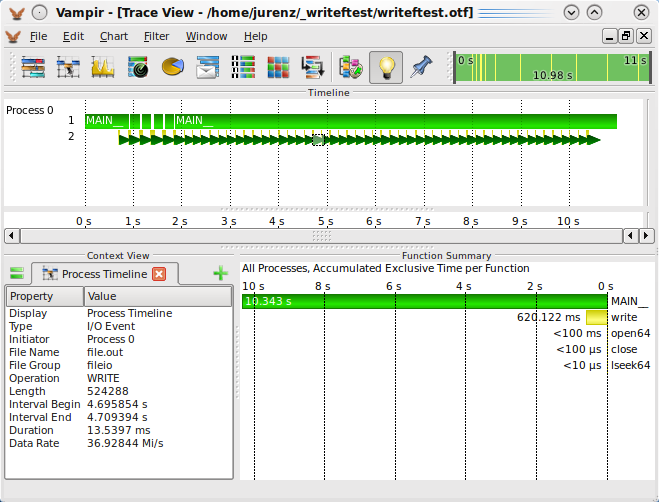
\includegraphics[width=10.5cm]{fortran_formatted_io.png}
\end{center}
\caption{This trace of a Fortran application shows many isolated I/O operations
and much time accounted to the MAIN function. Yet only a single formatted I/O
write operation is issued in the code. As VampirTrace is not able to trace the
Fortran I/O layer, it looks like the application itself uses cpu time between
the traced LIBC I/O operations, which does not reflect the actual happenings.}
\label{fig:fortran_io}
\end{figure}

\section[There is no *.otf file. What can I do?]{The application has run to completion, but there is no *.otf file. What can I do?}

The absence of an \texttt{*.otf} file usually means that the trace was not unified. This
is the case on certain platforms, e.g.~when using DYNINST or when the local traces
are not available when the application ends and VampirTrace performs trace unification.

In those cases, a \texttt{*.uctl} file can be found in the directory of the trace file and the
user needs to perform trace unification manually. See Sections~\ref{sec:unification} and~\ref{sec:VTUNIFY}
to learn more about using \texttt{vtunify}.

%\section{What limitations are associated with VT\_ON/VT\_OFF?}
\section{What limitations are associated with "on/off" and buffer rewind?}
\label{sec:faq_onoff}

Starting and stopping tracing by using the \texttt{VT\_ON/VT\_OFF} calls 
as well as the buffer rewind method are considered
advanced usage of VampirTrace and should be performed with care. When restarting
the recording of events, the call stack of the application has to have the same depth
as when the recording was stopped. The same applies for the rewind call, which
has to be at the same stack level as the rewind mark. If this is not the case, an error
message will be printed during runtime and VampirTrace will abort execution.
A safe method is to call \texttt{VT\_OFF} and \texttt{VT\_ON} in the same function.

It is allowed to use "on/off" in a section between a rewind mark and a buffer rewind call.
But it is not allowed to call \texttt{VT\_SET\_REWIND\_MARK} or \texttt{VT\_REWIND}
during a section deactivated by the "on/off" functionality.

Buffer flushes interfere with the rewind method: If the trace buffer is flushed
after the call to \texttt{VT\_SET\_REWIND\_MARK}, the mark is removed and a subsequent 
call to \texttt{VT\_REWIND} will not work and issue a warning message.

In addition, stopping or rewinding tracing while waiting for MPI messages can cause those MPI messages not to
be recorded in the trace. This can cause problems when analyzing the OTF trace afterwards, e.g.,~ with Vampir.


\section{VampirTrace warns that it ``cannot lock file a.lock'', what's wrong?}
\label{sec:faq_filelock}

For unique naming of multiple trace files in the same directory, a file \texttt{*.lock}
is created and locked for exclusive access if \texttt{VT\_FILE\_UNIQUE}
is set to \texttt{yes} (\rarr ~Section~\ref{sec:tracefilename}).
%If file locking is not implemented,
Some file systems do not implement file locking.
In this case, VampirTrace still tries to name the trace files uniquely, but this may fail
in certain cases.
Alternatively, you can manually control the unique file naming by setting 
\texttt{VT\_FILE\_UNIQUE} to a different numerical ID for each program run.

\section[Can I relocate my VampirTrace installation?]{Can I relocate my VampirTrace installation without rebuilding from source?}
\label{sec:faq_relocate}

VampirTrace hard-codes some directory paths in its executables and libraries based on installation
paths specified by the \texttt{configure} script. However, it's possible to move an existing VampirTrace
installation to another location and use it without rebuild from source.
Therefore it's necessary to set the environment variable \texttt{VT\_PREFIX} to the new installation prefix
before using VampirTrace's Compiler Wrappers (\rarr ~Section~\ref{sec:compiler_wrappers}) or launching an
instrumented application. For example:

\begin{verbatim}
./configure --prefix=/opt/vampirtrace
make install
mv /opt/vampirtrace $HOME/vampirtrace
export VT_PREFIX=$HOME/vampirtrace
\end{verbatim}

\section{What are the byte counts in collective communication records?}
\label{sec:faq_collective_bytes}

The byte counts in collective communication records changed with version 5.10.

From 5.10 on, the byte counts of collective communication records show the 
bytes per rank given to the MPI call or returned by the MPI call. 
This is the MPI API perspective. It is next to impossible to find out how many 
bytes are actually sent or received during a collective operation by any other 
MPI implementation.

In the past (until VampirTrace version 5.9), the byte count in collective 
operation records was defined differently. It used a simple and naive 
hypothetical implementation of collectives based on point-to-point messages 
and derived the byte counts from that. This might have been more confusing than
helpful and was therefore changed. 

Thanks to Eugene Loh for pointing this out!
 
\section{I get ``error: unknown asm constraint letter''}
\label{sec:faq_asm_error}

It is a known issue with the tau\_instrumentor that it doesn't support inline assembler code.
At the moment there is no other solution than using another kind of instrumentation like
compiler instrumenation (\rarr ~Section~\ref{sec:compinst}) or manual instrumenation (\rarr ~Section~\ref{sec:maninst}).

\section{I have a question that is not answered in this document!}
\label{sec:faq_unanswered}

You may contact us at \href{mailto:vampirsupport@zih.tu-dresden.de}{vampirsupport@zih.tu-dresden.de}
for support on installing and using VampirTrace.

\section{I need support for additional features so I can trace application xyz.}
\label{sec:faq_morefeatures}

Suggestions are always welcome (contact: \href{mailto:vampirsupport@zih.tu-dresden.de}{vampirsupport@zih.tu-dresden.de})
but there is a chance that we can not implement all your wishes as our resources
are limited.

Anyways, the source code of VampirTrace is open to everybody so you may
implement support for new stuff yourself.
If you provide us with your additions afterwards we will consider merging them
into the official VampirTrace package.
\end{latexonly}
\end{document}
 
